\section{Variable Objects in Astronomy}
\label{sec:theory-variable-objects}

When observing the sky over a sufficient time span, we empirically find that a lot of objects are subject to flux variability, \ie their observed magnitude $m$ is a function of time, even on short time--scales\footnote{Evidently, on the time span of their lifetime, all stars show some kind of variability as they evolve. However, this is not what we referd to by the term \emph{variability}.}. These significant changes in brightness can be somewhere between some thousandths of a magnitude and multiples of a magnitude. Some variables change very rapidly with periods of several hours, while others take years to complete one cycle. Some are strictly periodic, while others show rather stochastic, non--deterministic behaviour, which is much harder to characterise. It is important to realise that besides the simple periodic behaviour of some sources, there are also sources with periodic behaviour \emph{in--between} non--periodic behaviour, or even sources with multi--periodic behaviour with separate independent cycles such that, in the end, all we see as an observer is the superposition of several modes \citep{hanslmeier2007}.\\

% Elaborate more on motivation
A systematic observation of variables can provide valuable insight on cosmic evolution and stellar properties, such as temperature, mass and radius \citep{percy2007}. There are numerous types of variable objects with all kind of different mechanisms for variability. Ultimately, it all boils down to the reason for variability, which gives rise to different categories of variables. An exhaustive liste of variables is beyond the scope of this work, but we will try to 

% Can not explain all different classes in this work

\subsection{Intrinsic \& Extrinsic Variability}
\label{subsec:intrinsic-extrinsic-variability}

We say that an object shows \emph{intrinsic} variability, when the change in brightness is caused by real changes in the physical state of the object. Sources with intrinsic variability can be grouped into \emph{pulsating}, \emph{eruptive} and \emph{catalysmic} or \emph{explosive} variables.

\begin{itemize}
\item Pulsating variables are oscillating in radiative luminosity and radius $R$ because they are not in hydrostatic equilibrium
\begin{equation}
\label{eq:hydrostatic-equilibrium}
\frac{\mathrm{d}P}{\mathrm{d}R} \overset{!}= - \rho(R) \, \frac{G M(R)}{R^2},
\end{equation}
where $M$ is the star's mass within a sphere of radius $R$ and pressure $P$. The driving mechanism for radial pulsation in the instability strip is the $\kappa$-mechanism \citep{buchler1993}, which occurs if the opacity $\kappa$ within the stellar atmosphere increases with increasing temperature $T$ (at least in one layer), \ie $\kappa \propto T$. This will lead to the following effect: If $T$ and $P$ increase within a layer $\delta R$, the radiation pressure from within will increase as well, leading to an expansion of the layer, which in turn will lead to falling $T$ and $P$, directly resulting in decreasing $\kappa$. Since that will allow radiation to escape more easily, this will lead to a decrease in radiation pressure, which causes the layer to sink back in due to gravitation \citep{goodman2011}, where inertia restarts the cyle.\footnote{This is in fact somehwat simplified, because -- in general -- $\kappa$ will be a function of temperature $T$, pressure $P$ and wavelength $\lambda$. The actual mechanism inside the stars are more complicated and details are still subject to research. For a more exhaustive explanation see \citet{cox1980, percy2007}.} Another important cause for pulsation --- at least for very massive stars $\ge 100 \, \unit{M_\odot}$ \citep{buchler1993} --- is the $\epsilon$-mechanism, this time due to temperature and pressure dependent nuclear fusion energy generation rate $\epsilon(T, P)$.\\

There are a lot of different types of pulsating variables, but  some of the more important subclasses are:
	\begin{itemize}[label=$\circ$]
	\item \emph{Classical Cepheids} or \emph{$\delta$--Cepheids} are bright giant and supergiants with masses of $5$--$10 \, \unit{M_\odot}$, mostly in the helium--core--burning phase, that have periods between $1.0$--$50.0 \, \unit{d}$ \citep{cox1980}, and can be found in a diagonal, narrow strip in the Hertzsprung--Russell diagram known as the \emph{instability strip}. They belong certainly to the most important variables, because of their well established \emph{period--luminosity} relation
	\begin{equation}
	\label{eq:period-luminosity-relation}
	\cdots = \cdots,\footnote{This was discovered by Henrietta Swan Leavitt in the beginning of the $20^\text{th}$ century, who was a computer --- note the queer, original meaning of this word back then --- at the Harvard Observatory, by laborious, manual screening of photographic plates.}
	\end{equation}
	which allows astronomers, after proper calibration, to use Cepheids as \emph{standard candles} for distance estimation. Standard candles are objects with a known absolute magnitude $M$, which can then be used to calculate the distance modulus $\mu = m - M$ by measuring the apparent magnitude. The object's distance $d$ in $\unit{pc}$ is then given by solving
	\begin{equation}
	\log_{10}(d) = 1 + \frac{\mu}{5},
	\end{equation}
	assuming negligible interstellar absorption \citep{hanslmeier2007}. This turned out to be invaluable, and was an important contribution to astronomy.\todo{Insert equation}
	\item \emph{$\delta$-Scuti} stars or \emph{Dwarf Cepheids} are short--periodic ($0.7$--$5.0 \, \unit{h}$) variables with small amplitudes and typical masses of $1$--$2 \, \unit{M_\odot}$. They are usually multi--periodic and oscillate in both radial and non--radial modes, making them somewhat difficult to describe.
	% Dwarf cepheids
	\item \emph{RR Lyrae} are smaller, fainter objects than Cepheids. They have masses between $0.5$--$0.6 \, \unit{M_\odot}$ and typical periods between $0.2 $--$1.2 \, \unit{d}$ \citep{unsoeld2001}. Their phase and amplitude change over the course of the Blazhko cycle (\emph{Blazhko effect}) \citep{soszy2008}. Similar to Cepheids, RR Lyrae can be used as standard candles, although this will be harder for far away objects due to their fainter nature.
	% Also known as "cluster Cepheids" because they commonly occur in globular clusters
	\item \emph{Long--periodic variables} are rather cool pulsating stars with periods of $30$--$1000 \, \unit{d}$ and divide into \emph{Mira} and \emph{Semiregulars} with fairly irregular variability. Mira variables are red giants $\le 2 \, \unit{M_\odot}$ on the asymptotic giant branch (AGB) \citep{unsoeld2001} and were among the first discovered variables, which is --- at least to some extent --- due to the their high variability.
	% Mira, and Semiregulars
	\end{itemize}

\item{Blazhko effect for RRL}
\item Eruptive variables exhibit variability due to sudden, violent outbursts.
\item Catalysmic \& Explosive variables $\cdots$
\todo{Explain Catalysmic, explosive, eruoptive variables}
% Novae, Dward Novae and Supernovae

\todo{Add Blue variables}

\item \emph{Quasi--stellar objects} (QSOs) or \emph{quasars} (generally active galactic nuclei (AGN)) are extraordinary luminous ($10^{12}$--$10^{14} \, \unit{L_\odot}$), distant objects at the center of active galaxies. The emission of some $10^{40} \, \unit{W}$ is powered by the accretion of matter into supermassive black holes ($10^7$--$10^9 \, \unit{M_\odot}$) \citep{hanslmeier2007}. While being among the brightest objects in the observable universe over a broad range of the electromagnetic spectrum, most quasars appear faint from Earth, and can not be seen without special equipment. They show broad emission lines with a high redshift in their spectra (up to $z  = \Delta \lambda / \lambda_0 \approx 6$), which is due to the high velocities of the emitting gas. Most quasars show aperiodic photometric variability, and their change in brightness varies at $\approx 20\%$ on timescales of several months to years. Their smooth power spectra suggest a stochastic reason for variability \citep{macleod2010}, and it has been shown by \citet{kozlowski2010} that the observed light curves can be described by a \emph{damped random walk} (DRW).\todo{For the quasars: Add reference to structure function}

% Broad emission lines in spectra
% Rapid changes in luminosity in the optical range
% Powered by accretion disk
% Not much bigger than the solar system,  -> high density

\end{itemize}

On the other hand, if the change in brightness as perceived from the earth is merely due to external influences, a variable exhibits \emph{extrinsic} variability.

\begin{itemize}
\item Rotating variables change in brightness because their surface is not homogeneous, \eg has brighter and darker areas, that contribute accordingly to the overall brightness when rotating. One example for this is, of course, the Sun with its sunspots. For this type of variables, the amplitude changes are normally quite small.
\item Eclipsing binaries occur in binary star systems, where two stars are orbiting around some common centre of masse. Consequently, when observerd from the right angle, they show variability because one component of the systems is eclipsed by the other component. In their light curves, we can see two bumps, the primary eclipse and the secondary eclipse, which might only be a partial eclipse. In fact, the majority of stars in Milky Way are binary systems.
% Majority of stars in milkway are binary systems
% Primary eclipse and secondary eclipse
% Ask Kester for the reason why we see more short-periodic EB
\item Planetary transits could also block some of the light reaching the observer, leading to an overall decrease in brightness during the transit. This fact can be used, amongst others, to detect extrasolar planets (\emph{transit method}) orbiting distant stars.
\end{itemize}
 
% Pulsating variables 
% Cepheids 
% $\delta$--Scutis
% RR Lyrae
% Eclipsing binaries
% Active stars, flares and spots

\subsection{The Light Curves of Variable Stars}
\label{subsec:light-curves-variables}

\begin{figure}[H]
	\centering
	\begin{subfigure}[t]{0.49\textwidth}
		\centering
		\caption{Cepheid ($T_{\text{LS}} = 4.73 \, \unit{d}$)}
		\label{fig:lightcurve-ceph}
		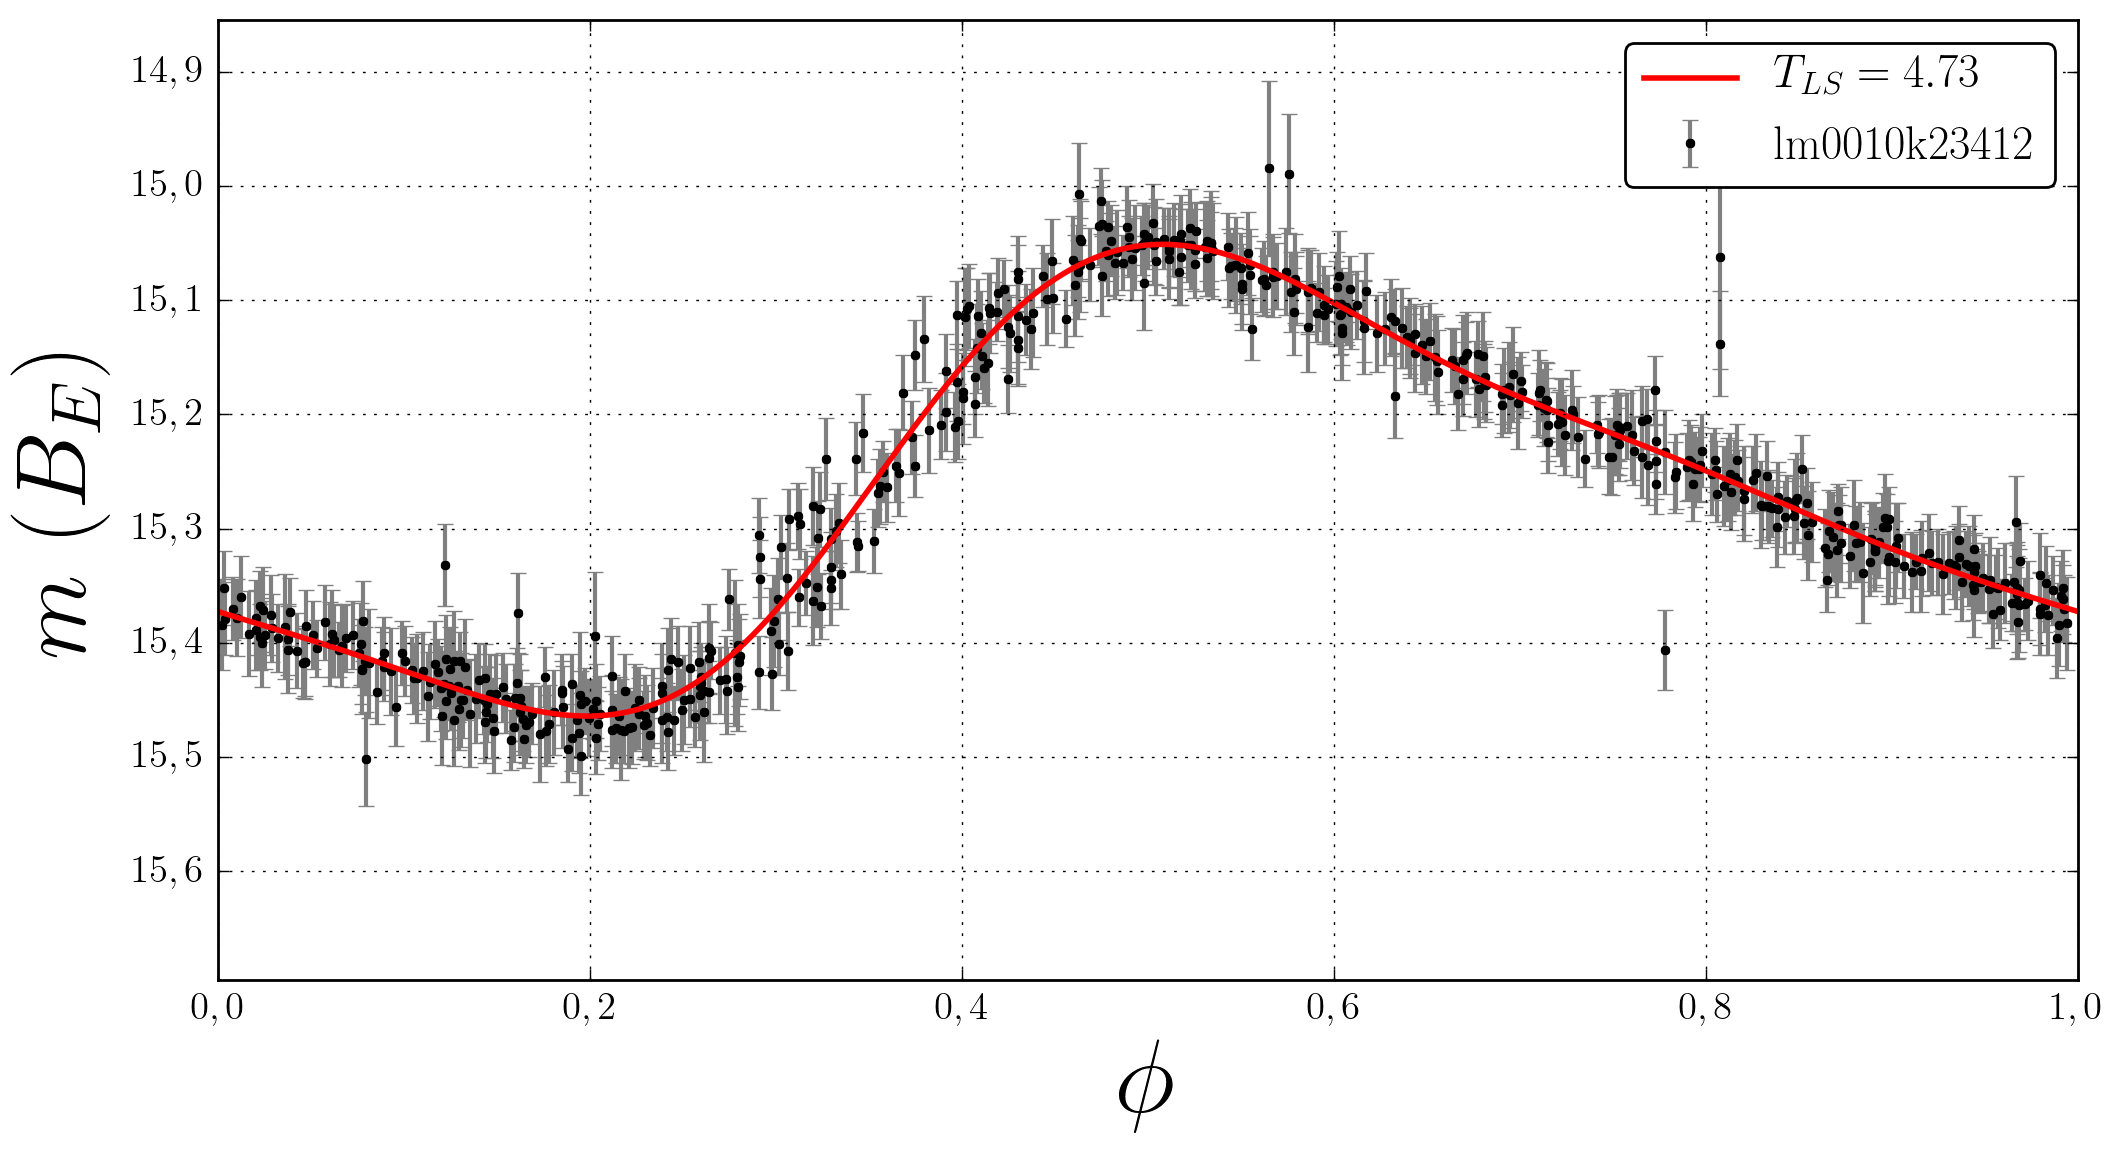
\includegraphics[width=\textwidth]{figures/lightcurves/ceph.png}				
	\end{subfigure}
	\begin{subfigure}[t]{0.49\textwidth}
		\centering
		\caption{Type II Cepheid ($T_{\text{LS}} = 12.69 \, \unit{d}$)}
		\label{fig:lightcurve-t2ceph}
		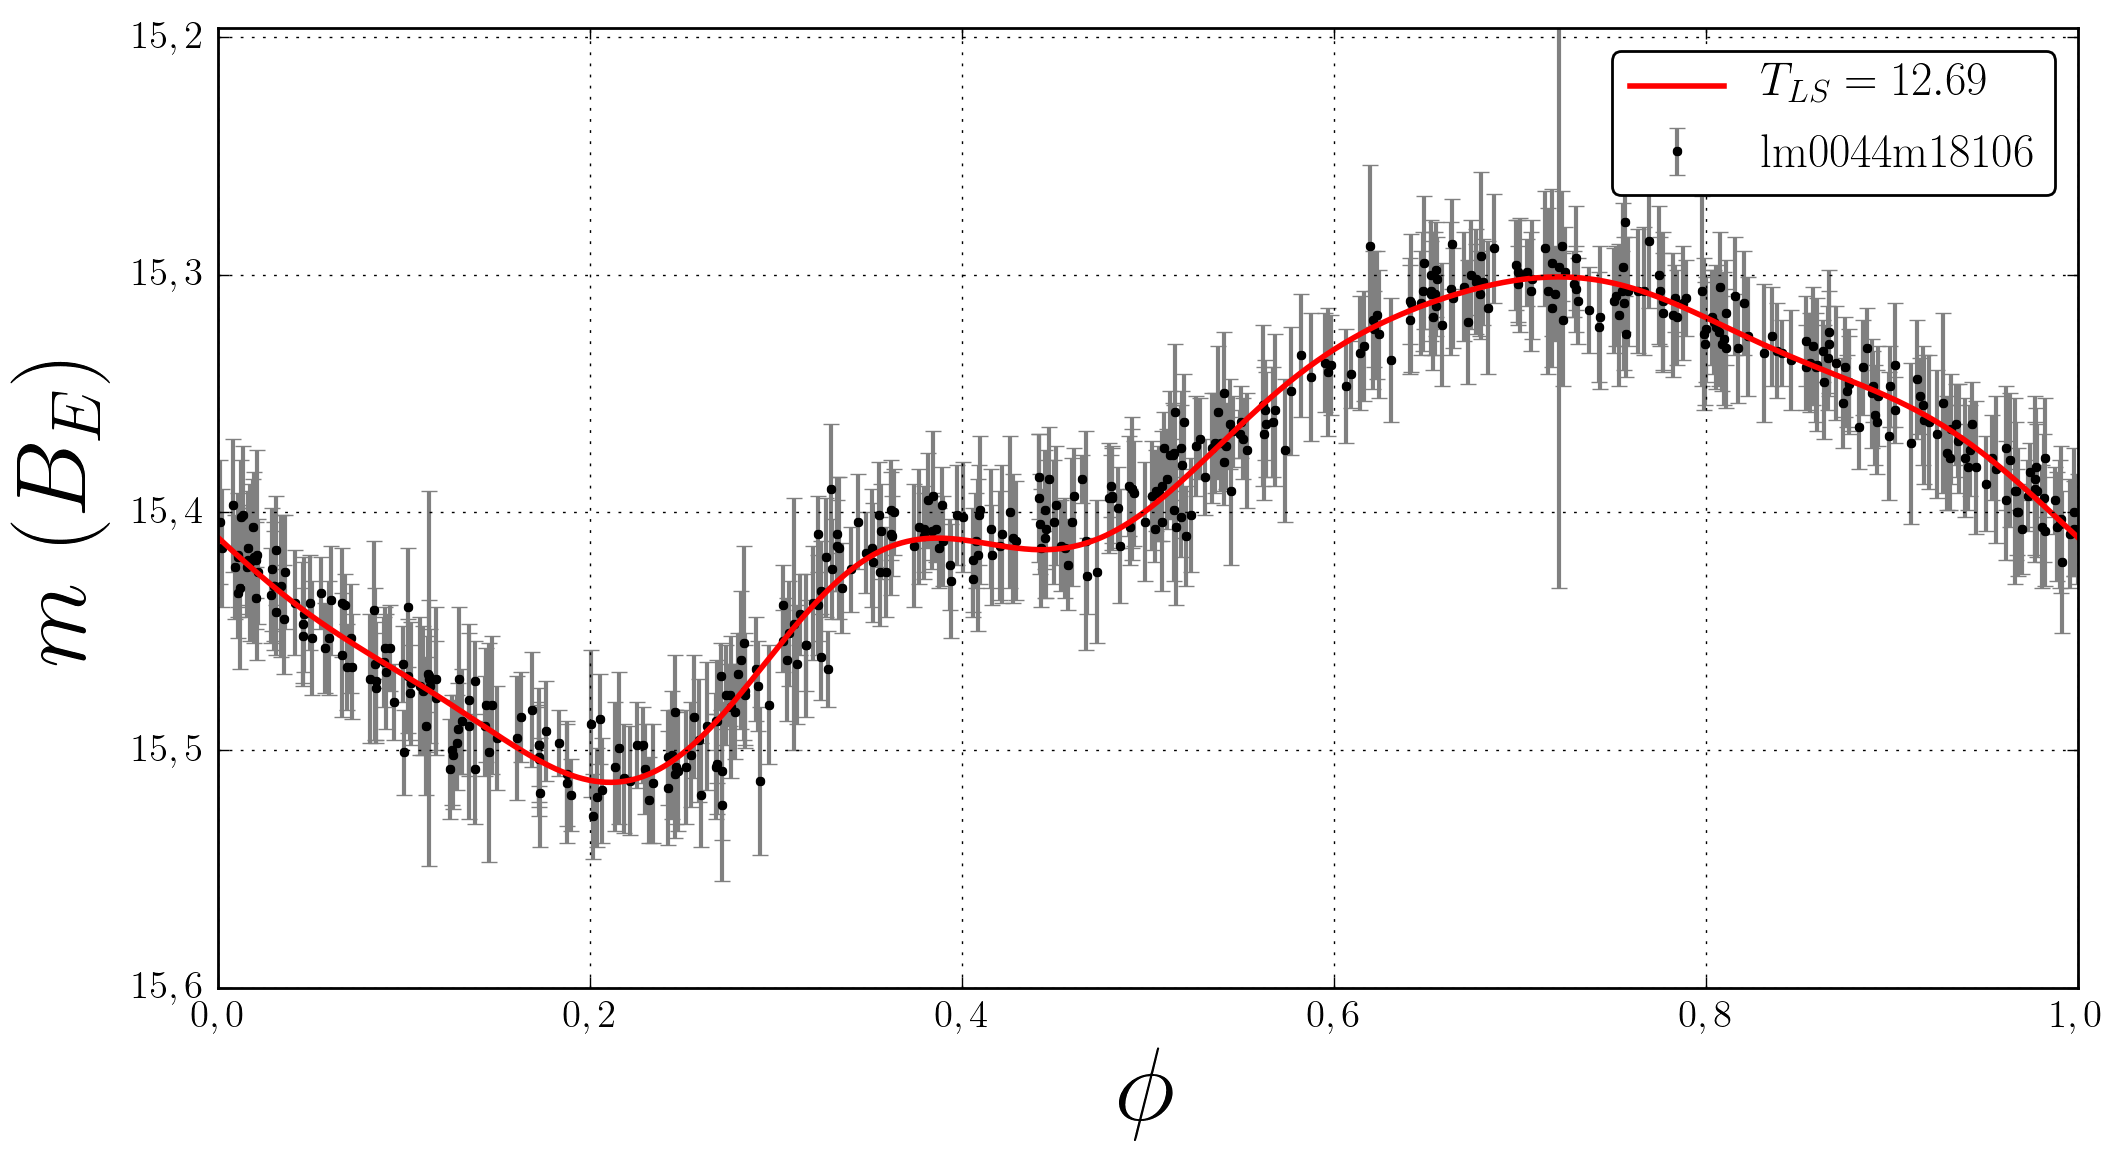
\includegraphics[width=\textwidth]{figures/lightcurves/t2ceph.png}				
	\end{subfigure}
	\begin{subfigure}[t]{0.49\textwidth}
		\centering
		\caption{RR Lyrae ($T_{\text{LS}} = 0.51 \, \unit{d}$)}
		\label{fig:lightcurve-rrl}
		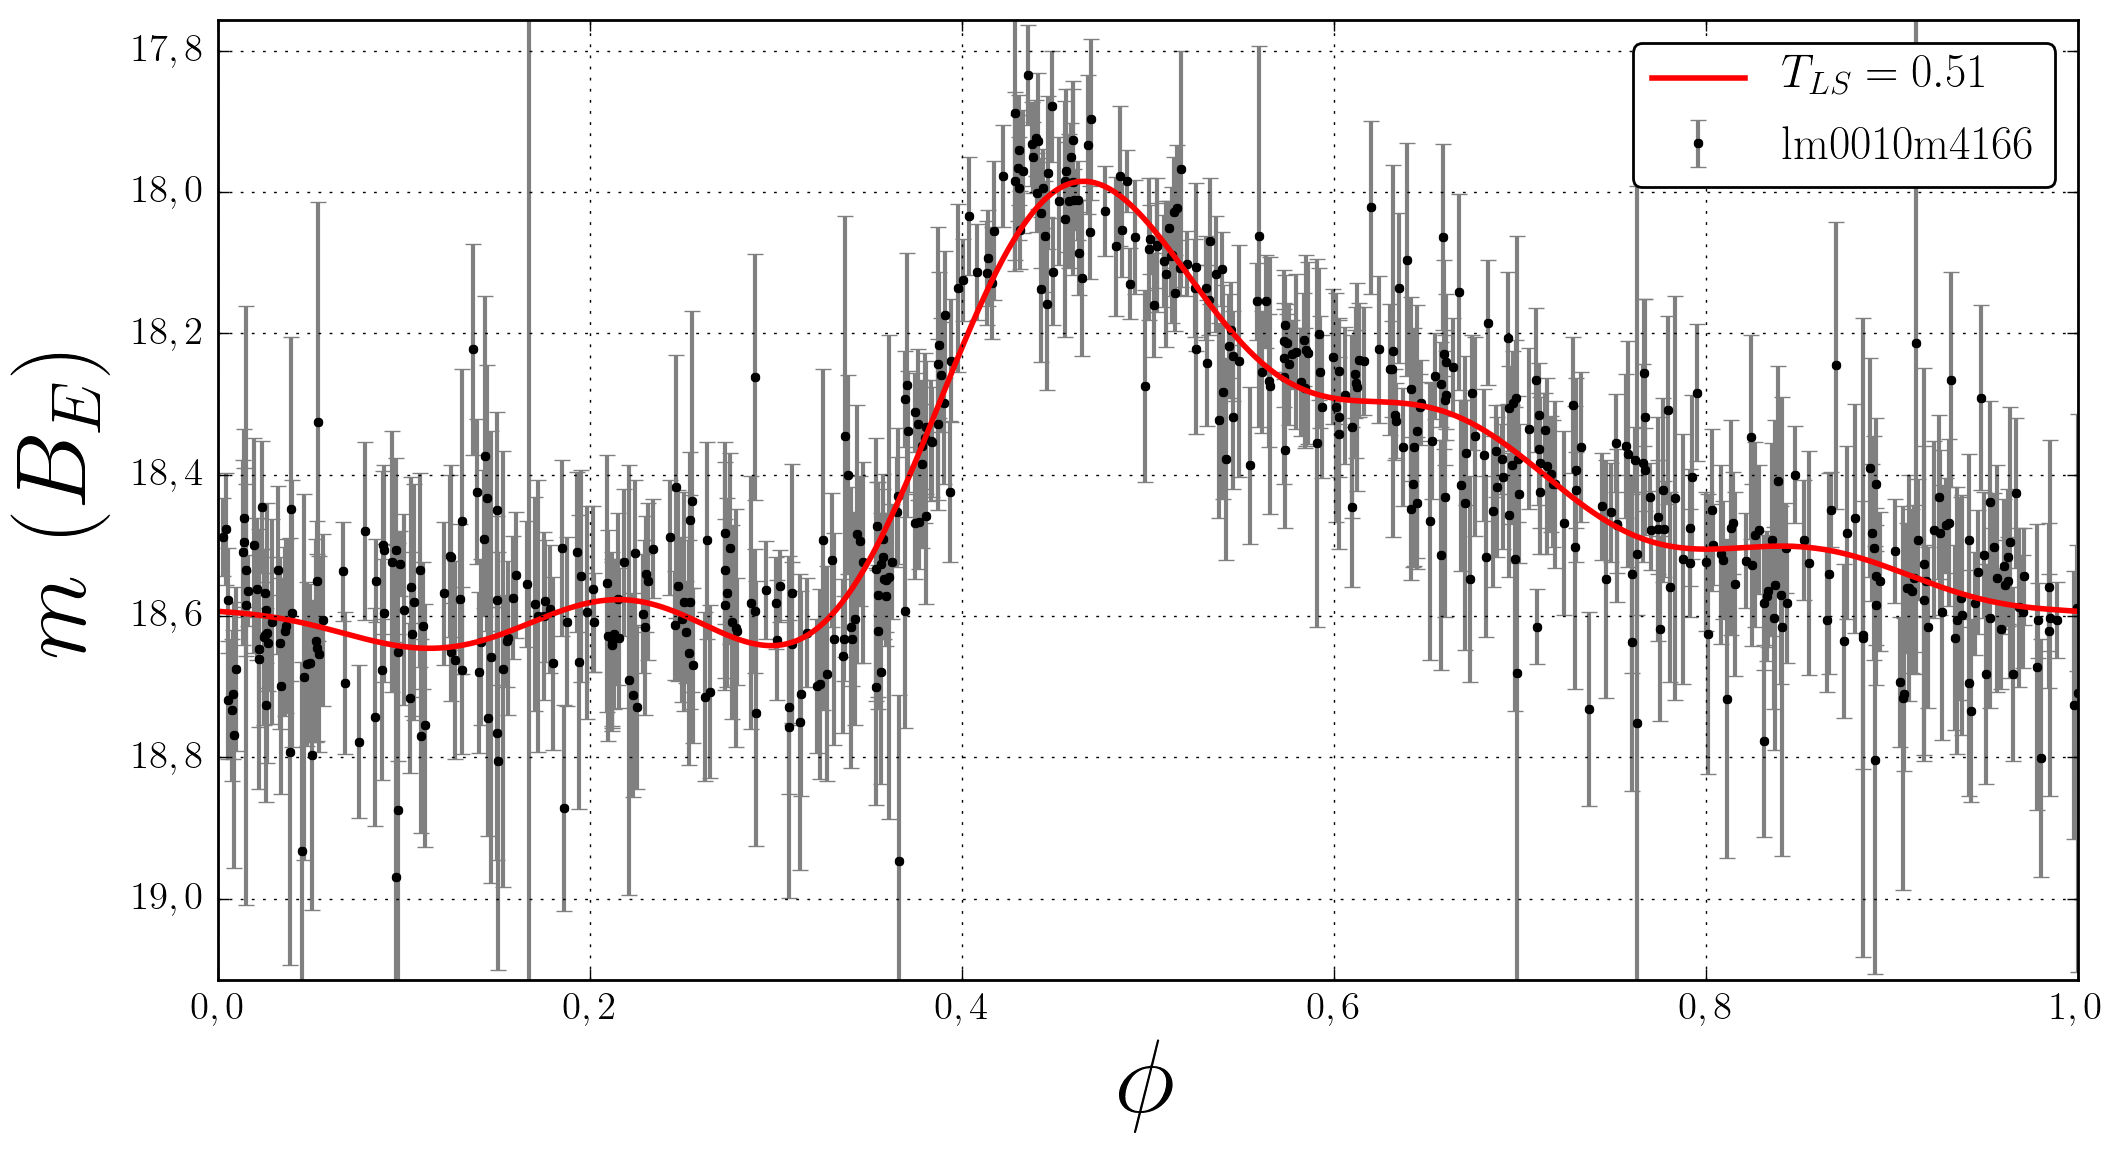
\includegraphics[width=\textwidth]{figures/lightcurves/rrl.png}		
	\end{subfigure}
	\begin{subfigure}[t]{0.49\textwidth}
		\centering
		\caption{$\delta$-Scuti ($T_{\text{LS}} = 0.06 \, \unit{d}$)}
		\label{fig:lightcurve-dsct}
		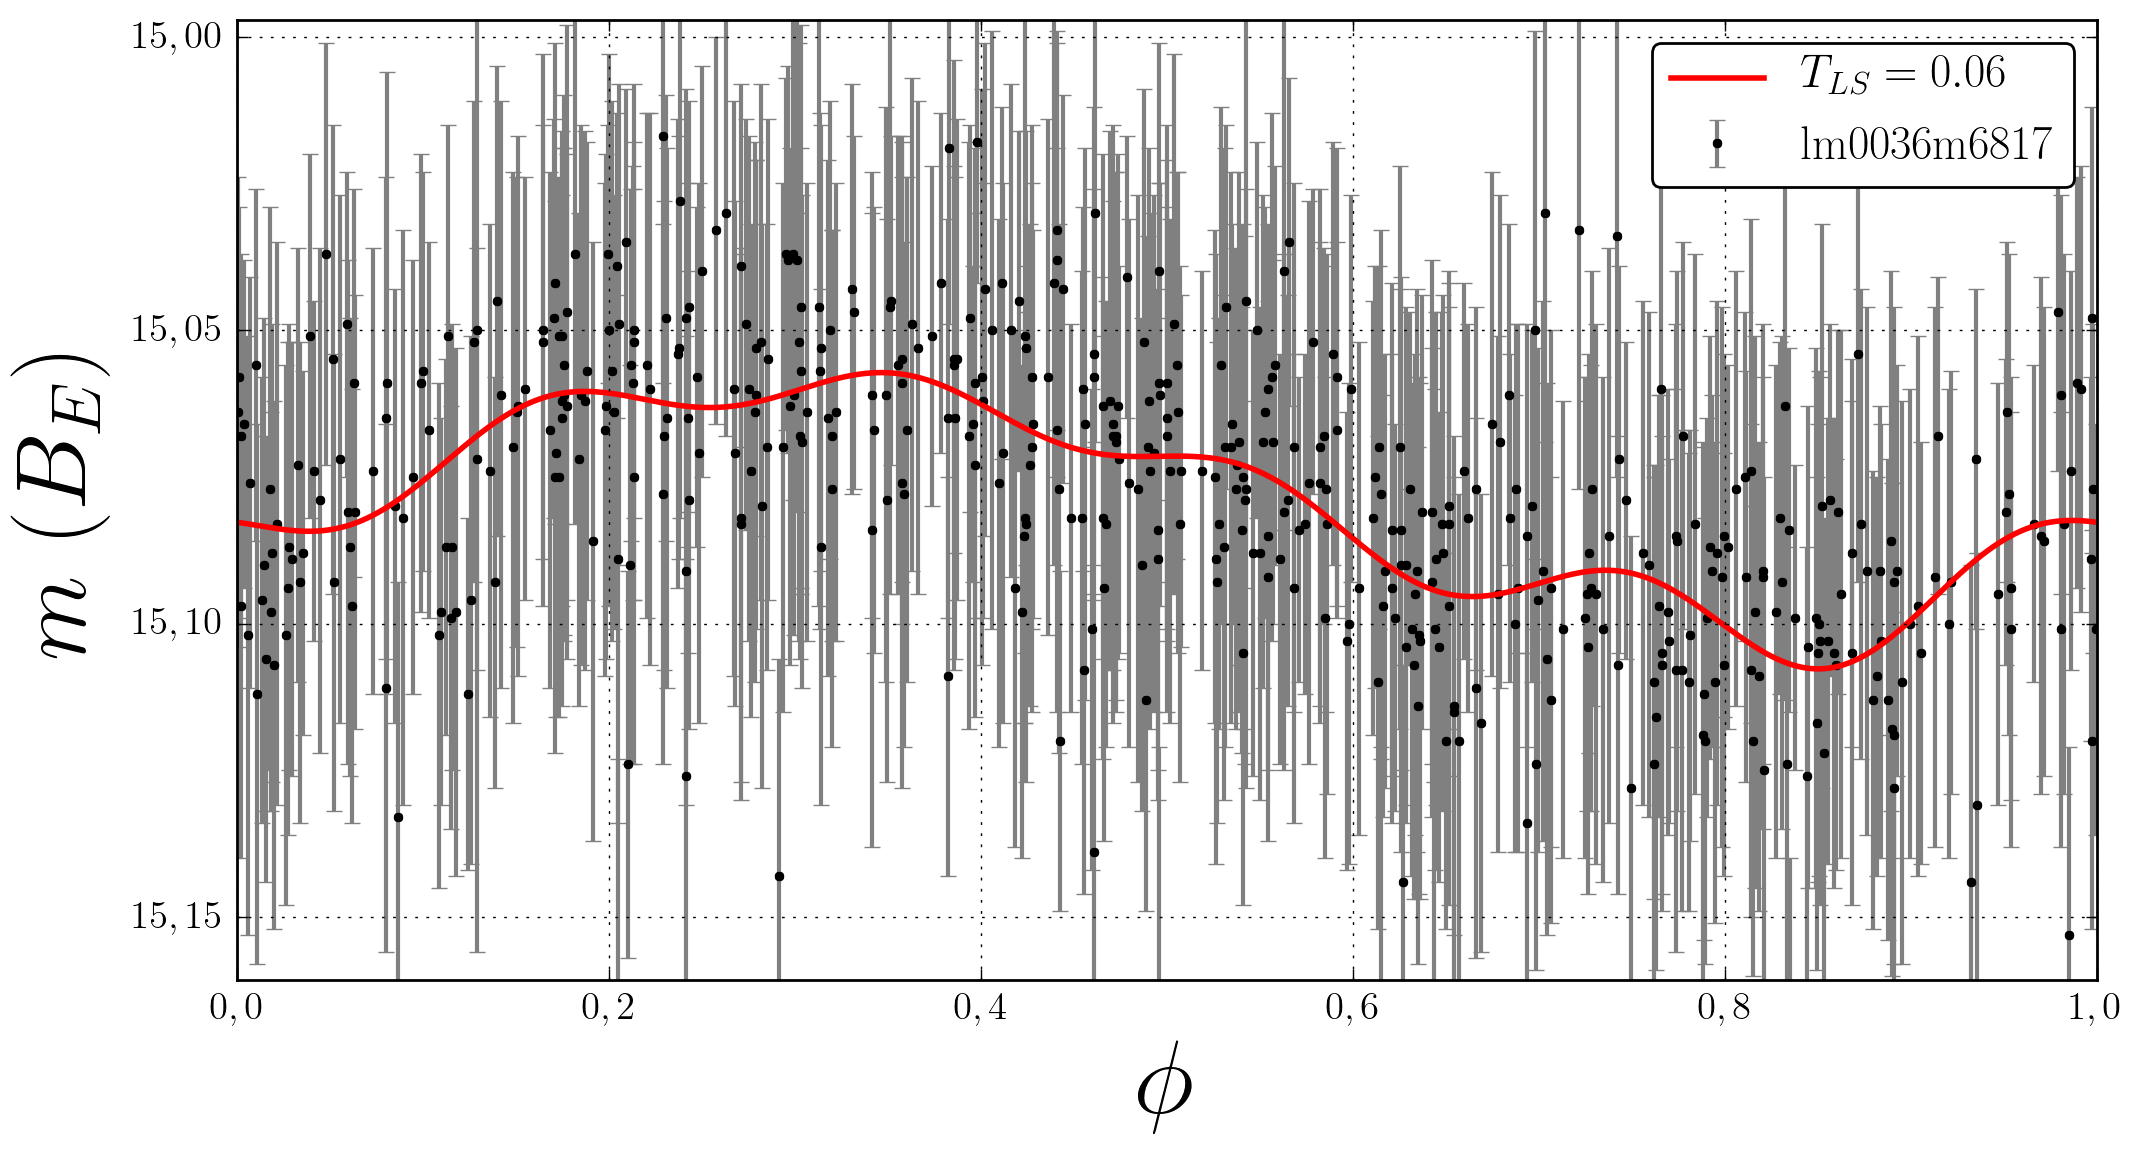
\includegraphics[width=\textwidth]{figures/lightcurves/dsct.png}		
	\end{subfigure}
	\begin{subfigure}[t]{0.49\textwidth}
		\centering
		\caption{Blue variable ($T_{\text{LS}} = 278.57 \, \unit{d}$)}
		\label{fig:lightcurve-bv}
		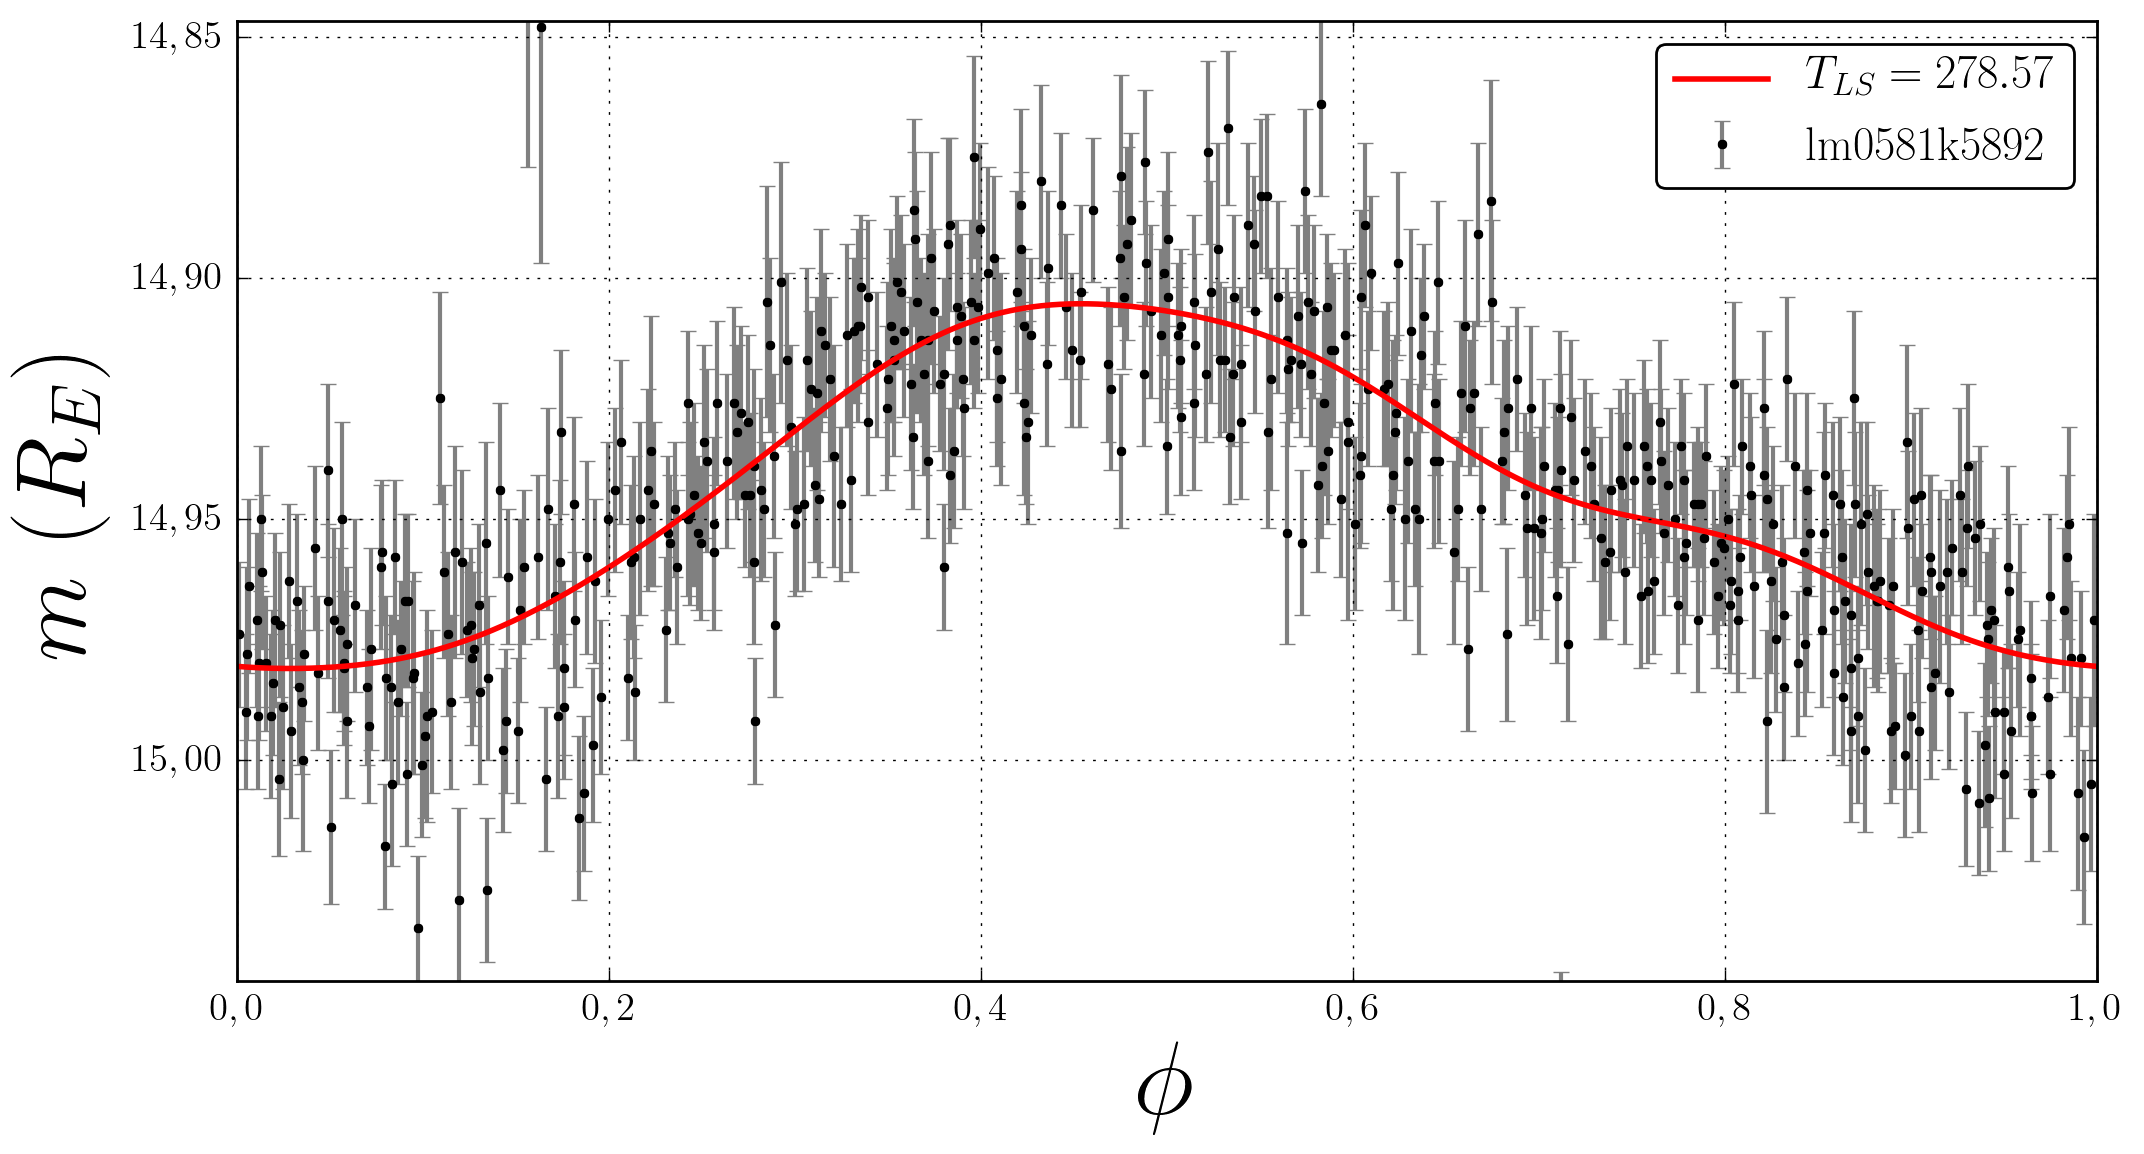
\includegraphics[width=\textwidth]{figures/lightcurves/bv.png}		
	\end{subfigure}
	\begin{subfigure}[t]{0.49\textwidth}
		\centering
		\caption{Long periodic variable ($T_{\text{LS}} = 430.82 \, \unit{d}$)}
		\label{fig:lightcurve-lpv}
		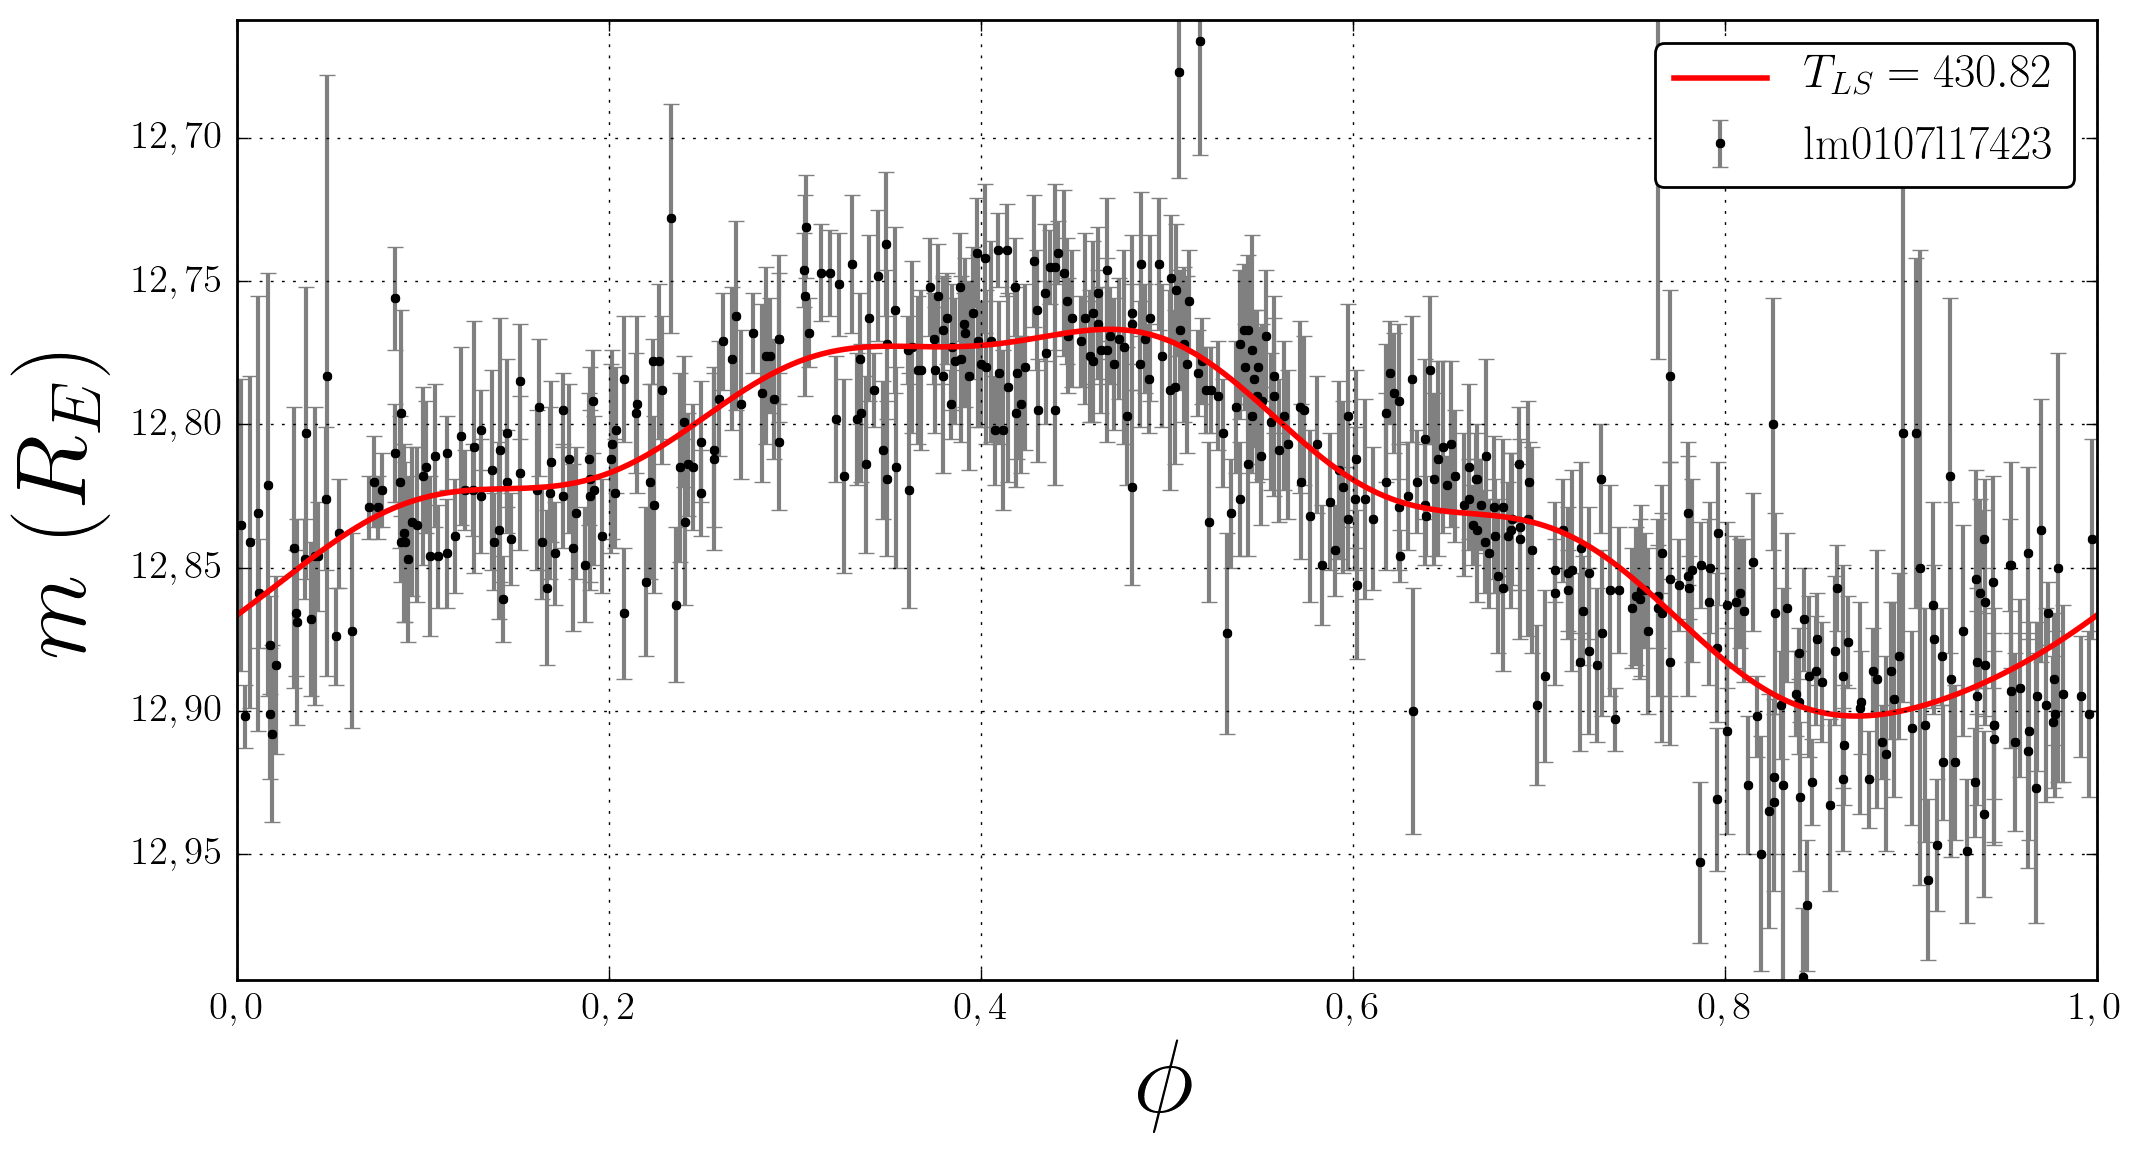
\includegraphics[width=\textwidth]{figures/lightcurves/lpv.png}		
	\end{subfigure}
	\begin{subfigure}[t]{0.49\textwidth}
		\centering
		\caption{Eclipsing binary ($T_{\text{LS}} = 0.83 \, \unit{d}$)}
		\label{fig:lightcurve-eb}
		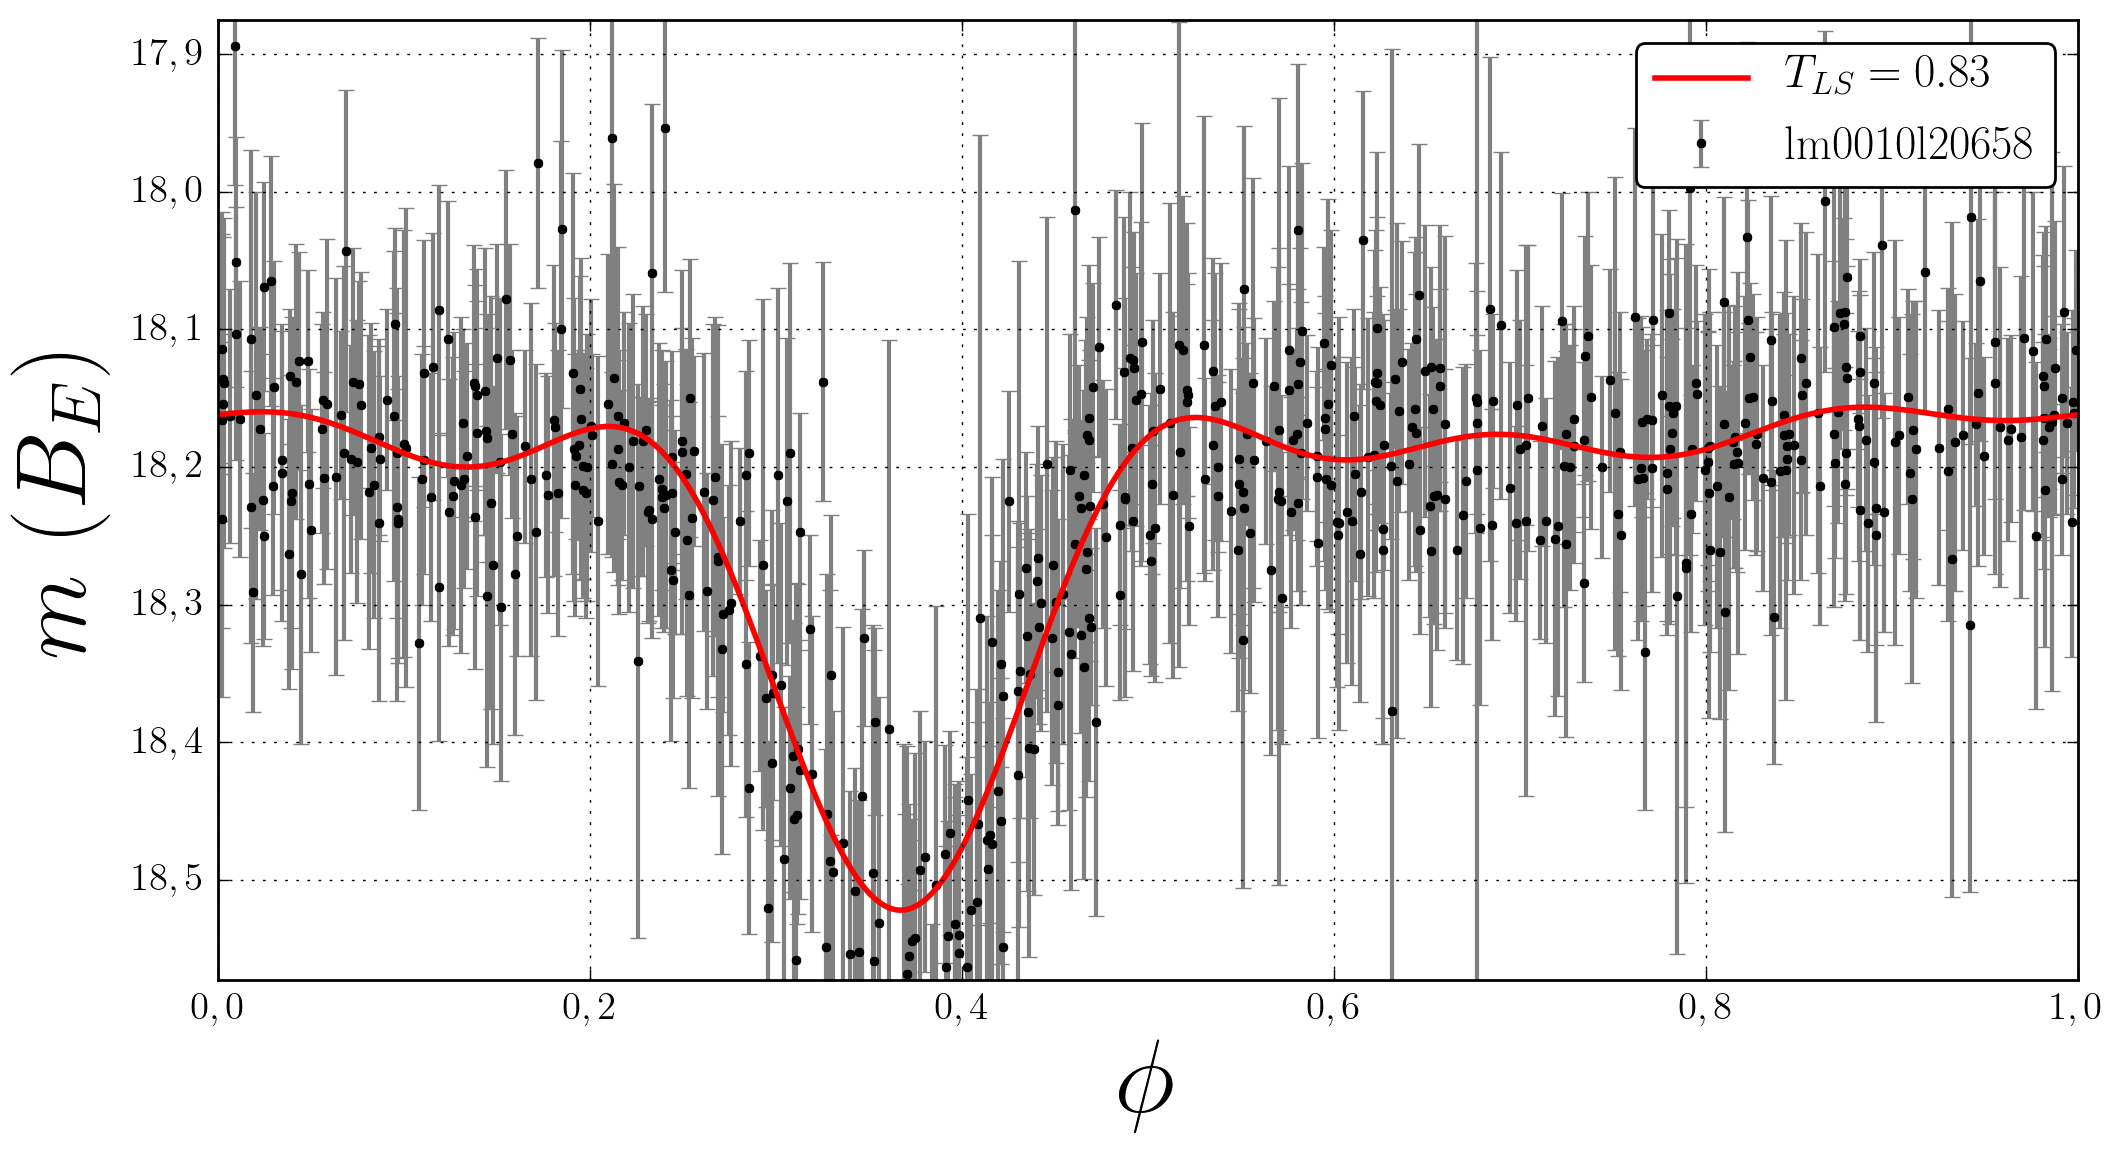
\includegraphics[width=\textwidth]{figures/lightcurves/eb.png}		
	\end{subfigure}
	\begin{subfigure}[t]{0.49\textwidth}
		\centering
		\caption{Quasar ($T_{\text{LS}} = 0.05 \, \unit{d}$)}
		\label{fig:lightcurve-qso}
		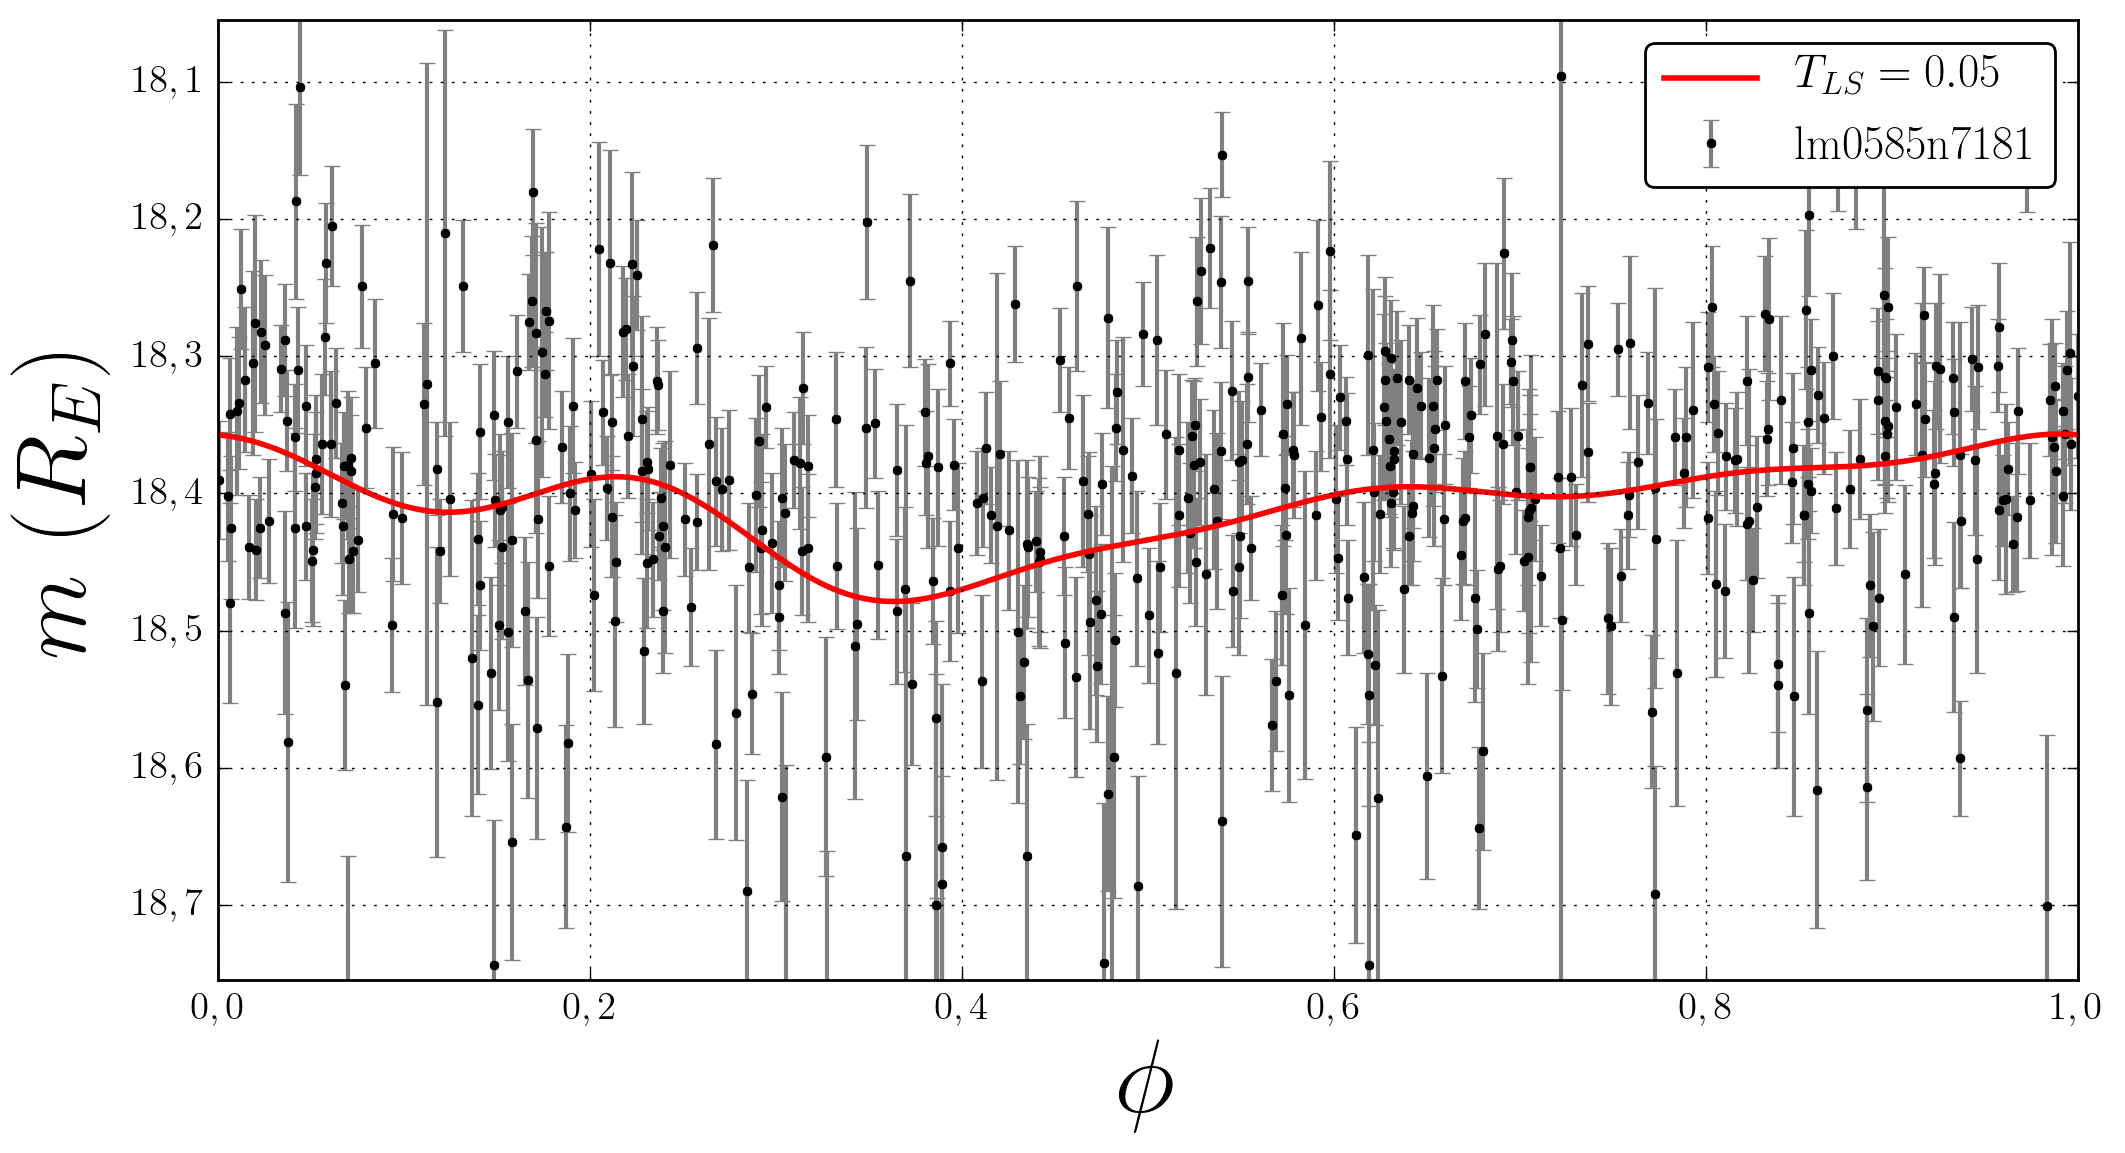
\includegraphics[width=\textwidth]{figures/lightcurves/qso.png}		
	\end{subfigure}
	\caption[Light curves for different variable sources]{This figure shows the phase--folded light curves of eight different variables, where the period was estimated with the Lomb--Scargle algorithm. The red lines indicate a five--term fourier series fit (see equation \eqref{eq:fourier-series-features}). Further comments on the individual light curve shapes can be found in the text.}
	\label{fig:various-light-curves}
\end{figure}
\todo{Check if LPV period is spurious}

\todo[inline]{Comment on the different light curve shapes}

In section \ref{subsec:intrinsic-extrinsic-variability}, we have seen that there are a whole variety of different mechanisms for variability. These mechanisms will lead to distinct light curves, giving rise to discriminative features that can later be used for classification. For the Cepheids (\ref{fig:lightcurve-ceph}), we can see a major change in brightness with small deviations. Although it is almost sinusoidal, we can clearly see that the decline is slower than the incline. The Type II Cepheids (\ref{fig:lightcurve-t2ceph}) show an extra bump in the light curve, which could be caused by a resonance between the different modes \citep{caputo1999}. The RR Lyrae (\ref{fig:lightcurve-rrl}) show a rapid increase followed by slower decline with some wiggles. The shape is clearly asymmetrical (which is not the case for RRc). $\delta$-Scuti's (\ref{fig:lightcurve-dsct}) light curves are in general similar to Cepheid's or RR Lyrae's, but with a much shorter period. Multi--mode oscillations are very common for $\delta$-Scuti. Blue variables (\ref{fig:lightcurve-bv}) show $\cdots$\todo{Describe BV light curve}. Long--periodic variables (\ref{fig:lightcurve-lpv}) have rather irregular, complicated light curves which is due to the fact that

\section{Statistical Analysis of Time Series}
\label{sec:statistical-analysis-time-series}

When observing one specific object over some time interval $\Delta t$, we can record its magnitude $m_i$ at time $t_i$ and obtain a so-called \emph{time series}. A time series $\Tau$ is a sequence of $N$ data points $(t_i, \vec y_i),\; t_i,(y_i)_j \in \mathbb{R}$ with $t_i < t_{i+1} \; \forall i = 1,\ldots,N$. We call $\Tau$ \emph{evenly--sampled} $\Leftrightarrow t_{i+1} - t_i = C \in \mathbb{R}$ where $C$ is constant. Otherwise, $\Tau$ is \emph{unevenly--sampled}.\\

\todo{Add definition of phase--fold}

\subsection{Algorithms for Period-finding}
\label{subsec:period-finding}

One very important feature of a periodic signal is, of course, its period $T$. However, reconstructing $T$ from the time series $\Tau$ is not trivial, especially if the data is very noisy. Ultimately, this is a regression problem itself, see subsection \ref{sec:introduction-machine-learning}, however, we will not tackle this with Machine Learning, but rather make use of some well--known methods devised for this very problem. The ultimate objective is to find the \emph{periodogram} $P(\omega)$ of signal, which is an estimator for the \emph{spectral density} $P$ as a function of the angular frequency $\omega = \frac{2 \pi}{T}$\footnote{In this regard, the periodogram can be seen as spectrum (some quantity over frequency) of a time series $\Tau$.}. Traditionally, there are a variety of methods available to characterize the signal in frequency--domain, mostly Fourier analysis. In 1898, Arthur Schuster defined the \emph{Schuster periodogram}

\begin{equation}
\label{eg:schuster-periodogram}
P_{\text{S}}(\omega) = \frac{1}{k} \, \biggl| \, \sum\limits_{i=1}^{k} y_i \euler^{-\mathrm{i} \omega t_i} \, \biggr|^2,
\end{equation}

% If omega0 is true period than e^{-i * omega0 * t_i} will have large contribution
% https://charlesmartin14.wordpress.com/2012/11/05/noisy-time-series/
% Reference for Schuster periodogram

for a time series $(t_i, y_i)$ of length $k$. Note that equation \eqref{eg:schuster-periodogram} is essentially given by $\| \mathcal{F}(\omega) \|_2 $, the $L^2$ norm of the discrete Fourier transform (DFT) $\mathcal{F}$ of the signal. Therefore, $P_{\text{S}}(\omega)$ can be approximated very efficiently when using the fast Fourier transform algorithm (FFT) \citep{cooley1965}, which allows for a runtime complexity of $\mathcal{O}(N\log{(N)})$ instead of $\mathcal{O}(N^2)$. However, it can be shown that those Fourier transform--based methods perform poorly on unevenly--sampled data, because they tend to boost long--periodic noise\todo{Explain long--periodic noise}. Since evenly--sampled data can be difficult to obtain, especially for earth--bound surveys in astronomy, a lot of effort was put into developing suitable methods that can cope with this kind of data. This work makes use of two popular methods devised for unevenly--sampled data, one based on least--squares spectral analysis (LSSA), namely the \emph{Lomb--Scargle periodogram}, and the other one based on the minimization of some metric for dispersion in phase space, in this case \emph{conditional entropy}. We provide a brief overview for both of them.

\subsubsection{Lomb--Scargle Periodogram}
\label{subsubsec:lomb-scargle}

The most prominent method for finding the period of an unevenly--sampled light curve was developed by \citet{lomb1976} and extended by \citet{scargle1982}. It is devised to find the period of a sinusoidal-shaped periodic signal. For a given time--series $(t_i, (y_i, \sigma_i))$ of length $k$ with arithmetic mean $\mu_y$ and variance of the noise $\sigma_y^2$, Scargle defines the \emph{normalized Lomb--Scargle periodogram} as

\begin{equation}
\label{eq:normalized-lomb-scargle}
P^{\text{N}}_{\text{LS}}(\omega) = \frac{1}{2 \sigma_y^2} \Bigg\{ \frac{\big[\sum\limits_{i=1}^k (y_i - \mu_y) \cos(\omega(t_i - \tau))\big]^2}{\sum\limits_{i=1}^k \cos^2(\omega(t_i - \tau))} + \frac{\big[\sum\limits_{i=1}^k (y_i - \mu_y) \sin(\omega(t_i - \tau))\big]^2}{\sum\limits_{i=1}^k \sin^2(\omega(t_i - \tau))}\Bigg\},
\end{equation}

where $\tau$ is a time--offset defined by

\begin{equation}
\tan(2 \omega \tau) = \frac{\sum\limits_{i=1}^k \sin(2 \omega t_i)}{\sum\limits_{i=1}^k \cos(2 \omega t_i)},
\end{equation}

which makes the periodogram $P^{\text{N}}_{\text{LS}}(\omega)$ invariant for a translation in $t$. Furthermore, this time--offset $\tau$ makes the periodogram identical to least--squares fitting of a single--component sinusoidal model of the form $y(t) = A \sin(\omega t + \varphi)$ \citep{horne1986, vanderplas2015}. Additionally it can be shown that --- if the periodogram is properly normalized\footnote{There has been a lively discussion about the correct normalization of the periodogram, which retains above convenient statistical properties, see \citet{lomb1976,astroML,zechmeister2009}. The correct normalization factor in equation \eqref{eq:normalized-lomb-scargle} is \emph{the total variance of the data}, as explained in detail in \citet{horne1986}.} --- $P^{\text{N}}_{\text{LS}}(\omega_0) \propto \exp(-x)$ for pure noise at any frequency $\omega_0$, where $x$ denotes the height of the peak. This exponential probability distribution gives rise to the \emph{false--alarm-probability (FAP)},

\begin{equation}
\text{FAP}_{\text{LS}}(x) = 1 - (1 - \euler^{-x})^M,
\end{equation}

which is a suitable and convenient estimator for the significance\footnote{In this case: The probability that the peak is the product of a true signal, rather than the result of randomly distributed noise.} of a peak, and can be identified as the probability that a peak of at least height $x$ will occur in a periodogram on a grid of $M$ independent frequencies \emph{when evaluated on pure noise} \citep{horne1986}.\\

In spite of its usefulness, there are some drawbacks of the normalized Lomb--Scargle periodogram in its original formulation:

\begin{itemize}
\item $P^{\text{N}}_{\text{LS}}(\omega)$ given by equation \eqref{eq:normalized-lomb-scargle} does not account for measurement errors, \eg by introducing weights for all data points. This however ignores an important aspect of the measurement process, where some data points might in fact be more accurate than others, for example due to changing conditions in the measurement environment.
\item Offset $\cdots$ % @TODO: Elaborate on constant offset
\end{itemize}

\todo[inline]{Add info about Generalized Lomb--Scargle}

% This led to further generalization...
% The \emph{generalized Lomb--Scargle periodogram} is less prone to aliasing, and provides more accurate results (http://arxiv.org/abs/0901.2573).

% Generalized and classical
% Bayesian generalized Lomb-Scargle (Martiniee)
% Single point estimate rather than a posterior probability distribution
% Multi-band periodogram and matrix formalism
% It is possible to carefully correct for such aliasing by iteratively removing contributions from the estimated window function (e.g. Roberts et al.1987), we’ll ignore this detail in the current work.
% Discrete and continous, Fast Fourier Transformation (FFT)
% Remarks concerning runtime N^2 and Nlog(N) implementations

\subsubsection{Conditional Entropy Periodogram}
\label{subsubsec:conditional-entropy}

Using conditional entropy for period finding was first proposed by \citet{graham2013} as an extension of a similar algorithm developed by \citet{cincotta1995}. Both algorithms look at the problem from an information--theoretic point of view. The fundamental idea is that the phase--folded light curve will form the most ordered, compact arrangement of points in phase space when folded with the true period, whereas it would look very noisy for most other periods. One way to quantify this would be to partition the $m$-$\phi$-plane into $k$ bins for each candidate period $\hat T_i$, and then calculating the \emph{Shannon entropy}

\todo{Maybe rename H to E for entropy}
\todo{Occupy a unit square}

\begin{equation}
\label{eq:shannon-entropy}
H_S = - \sum_{i=1}^k \mu_i \ln(\mu_i),
\end{equation}

where $\mu_i = \frac{n_i}{N}$ denotes the occupation probability for the $i^\text{th}$ bin, which is simply the number of data points in the $i^\text{th}$ bin $n_i$ over the total number of data points $N$. The best estimate of the true period $T$ would then be the candidate period $\hat T_i$ which minimizes equation \eqref{eq:shannon-entropy}. It has been established that this does not yield satisfying results on real--world data \citep{cincotta1999}, because the resulting periods are very often corresponding to the mean solar day $T_\odot = 1.00274 \, \unit{d}$. This effect can be corrected for to some extend, \eg by a wise choice of the partitioning as \citet{cincotta1999,drake2013}. For this reason \citeauthor{graham2013} devised their enhancement by proposing to substitute equation \eqref{eq:shannon-entropy} with the \emph{conditional entropy}

\begin{equation}
H_c = \sum_{i,j} p(m_i, \phi_i) \ln\big(\frac{p(\phi_j)}{p(m_i, \phi_j)}\big),
\end{equation}

where 

\todo[inline]{Add more about conditional entropy}

% Works good for evenly sampled datapoints

%We provide a runtime--optimized, fast \emph{Cython} implementation of the conditional entropy period--finding algorithm.

\subsection{Structure Function \& Stochastic Variability}
\label{subsec:structure-function}

As we have seen in section \ref{sec:theory-variable-objects}, quasars change their luminosity in a chaotic, stochastic manner. The precise physical cause for this variability is subject to ongoing research. \citet{pereyra2006} and \citet{li2008} present evidence that the variability is caused by a variable accretion rate $\dot M$. On the other hand, \citet{blackburne2010} demonstrate that a change in the effective area of the accretion disk could contribute to the overall variability. Regardless of the actual cause, we can describe QSO observations, \eg light curves, in a statistical manner. Structure function $\text{SF}$ analysis \citep{hughes1992,collier2001} is one way to do this, and has been shown (\eg \citet{schmidt2010}) to provide robust results in separating quasars from other variables sources. It characterizes the intrinsic, stochastic variability of a source by quantifing the variability amplitude $V$ of an object as a function of the time lag $\Delta t_{ij}$ between two observations $m_i, m_j$. This can be done for a large ensemble of sources, to analyse the properties of an entire population, or, if proper sampling is available, for individual objects. Given a magnitude time series of length $N$, we build a list of the $\frac{N(N-1)}{2}$ data pairs, and estimate the variability by

\begin{equation}
V_{ij}(\Delta t_{ij}) = \Delta m_{ij} - \sqrt{\sigma_i + \sigma_j},
\end{equation}

where the last term corrects for the photometric measurement errors, and $\Delta m_{ij}$ is the magnitude difference $m_i - m_j$. It is important to note that $\Delta t_{ij}$ denotes the time lag in the observed frame and \emph{not} in the object's rest frame. In principle, we could correct for this if further knowledge about the object's red shift was available. We then define the binned structure function as

\begin{equation}
\text{SF}(\Delta t) = \big\langle \sqrt{\frac{\pi}{2}} \big| \Delta m_{ij}  \big| - \sqrt{\sigma_{m_i}^2 + \sigma_{m_j}^2} \big\rangle_{\Delta \tau},
\label{eq:binned-structure-function}
\end{equation}

where $\langle \cdot \rangle_{\Delta \tau}$ is the arithmetic mean of all data points within bin $\Delta \tau$.\footnote{There are a lot of different definitions of equation \eqref{eq:binned-structure-function} We decide to follow \citet{schmidt2010}.} It has been established \citep{richards2006} that a power--law model of the form

\begin{equation}
A \, \big(\frac{\Delta t}{1 \, \unit{yr}}\big)^\gamma
\end{equation}

provides a decent fit for \eqref{eq:binned-structure-function}, where $A$ is an estimate of the root--mean--square magnitude variability on the timescale of $1 \, \unit{yr}$ and $\gamma$ is the logarithmic gradient of the change in magnitude.

\section{Statistical Inference Using Machine Learning}

\subsection{Introduction to Machine Learning}
\label{sec:introduction-machine-learning}

Machine Learning (ML), sometimes referred to as \emph{pattern recognition}, is a subfield of Artificial Intelligence (AI) primarily dealing with automated approaches to infer meaning from data in such a way that, after some training process, a model is obtained, that can later be used to make predictions or decisions on similar data or achieve some other kind of insight. This is a form of learning, because rather than explicitly programming certain decision rules, we want to generalize observations towards an underlying model that performs as well as possible when confronted with new data.\\

% @TODO: Elaborate on reinforcement learning
Depending on the problem to be solved and the data available, machine learning algorithms can be divided into \emph{supervised}, \emph{unsupervised}, \emph{reinforcement} learning and some hybrid form of these. In supervised learning, we train our model by providing examples of the desired output, whereas in unsupervised learning, $\cdots$. Reinforcement learning works by $\cdots$.\\

There are a variety of learning problems, such as \emph{classification problems}, \emph{regression problems} and \emph{clustering}, but also \emph{dimensionality reduction} and \emph{density estimation} are subject to Machine Learning.\\

% Explain classification, regression and clustering
% Describe supervised, unsupervised and reinforcment learning
% Large amounts of data, computationally efficient
% Elaborate on why machine learning vs. directly programming decision rules
% Also to given insight: Sometimes humans can not really describe how they are doing things
% Overfitting, underfitting
% Add some examples for machine learning problems

Please note that in practise both $N$ and $d$ can be very large, and inferring $\varphi$ from $\trainingdata$ directly can become computationally expensive or even unfeasible.

\subsubsection{Classification \& Regression}

In this work, we are primarily interested in classification and regression using supervised methods. Therefore, we are typically trying to solve the following problem: Given some training data

\begin{equation}
\trainingdata = \{ (\vec x_i, y_i) \where \vec x_i \in \mathbb{R}^d, y_i \in \classes \quad \forall i = 1,\ldots,N \},
\end{equation}

consisting of $N$ \emph{feature} vectors $\vec x_i \in \observations$ of length $d$ and $N$ \emph{labels} or \emph{classes} $y_i \in \classes$, find some mapping function $\varphi \colon \observations \to \classes$ such that

\begin{equation}
\estimator(\vec x_i) = y_i \in \classes \quad \forall i = 1,\ldots,N,
\end{equation}

where $y_i$ denotes the true class of an arbitrary observation $\vec x$ out of all possible observations $\observations$. In any case, $\varphi$ is an \emph{estimator}. If the label $y_i$ is a discrete value, $\varphi$ will be called \emph{classifier}, if it is continuous, $\varphi$ will be called \emph{regressor}.\footnote{The term \emph{probabilistic classifier} stands for an estimator that assigns a probability $p_{\text{class}}$ for every class to the input vector. Based on this, classification can be conducted, \eg by maximum likelihood.} We consider $\varphi$ to be optimal if, confronted with some testing data,

\begin{equation}
\testingdata = \{ (\vec x'_j) \where \vec x'_j \in \mathbb{R}^d \quad \forall j = 1,\ldots,N \},
\end{equation}

the estimator yields

\begin{equation}
\hat y_j := \varphi({\vec x'_j}) = y_j \quad \forall j = 1,\ldots,N,
\end{equation}

where $\hat y_j$ is the estimators response, and $y_j$ denotes the true class of $\vec x'_j$.

\subsubsection{Evaluating Models}

\todo{Write about generalization, overfitting, underfitting}
\todo{Write about $F_1$-score and weights...}

The estimators performance can be assessed by a variety of metrics: For classification, we define accuracy $A$, precision $P$ and recall $R$ as

\begin{equation}
A = \frac{T_p + T_n}{T_p + F_p + T_n + F_n}, \; P = \frac{T_p}{T_p + F_p}, \; R = \frac{T_p}{T_p + F_n},
\end{equation}

% @TODO: Elaborate on model evaluation

where $T_p, F_p, T_n, F_n$ denote the number of \emph{true positives}, \emph{false positives}, \emph{true negatives} and \emph{false negatives}\footnote{Accuracy, precision and recall are sometimes also referred to as \emph{}, \emph{}, \emph{}}. For regression, we usually want to minimize some suitable loss-function $L$.

\subsection{Algorithms for Classification \& Regression}
\label{subsec:algorithms-classification-and-regression}
\subsubsection{Support Vector Classifiers \& SVMs}

Support Vector Machines (SVMs)\footnote{A note to the terminology: Most literature refers to the linearly separable case as \emph{Support Vector classifier}, whereas the non--linear high--dimensional enhancement, incorporating kernel methods, are called \emph{Support Vector Machine}.}, originally proposed by \citet{vapnik1963} as linear classification, later extended by \citet{cortes1995} to allow for non--linear classification, are among the most common classification algorithms, especially for high--dimensional datasets. The underlying idea is to find a special \emph{hyperplane} $\hyperplane$, which will act as decision boundary in feature space $\featurespace$.\footnote{This is somewhat similar to \emph{perceptron learning} as devised by \citet{rosenblatt1958}. His algorithm however tries to find a separating hyperplane that minimizes the distance of misclassified points to the decision boundary \citep{hastie2001}.} Among all possible hyperplanes, the SVM decision boundary will be given by the hyperplane which separates the classes \emph{and} maximizes the distance to the closest data points for both classes, therefore called \emph{maximum--margin hyperplane} $\hat \hyperplane$. The data points on the decision boundary are \emph{support vectors}. In any case, $\hat \hyperplane$ is obtained by solving some kind of optimization problem. In the following we will assume that we are dealing with $d$-dimensional training data $\trainingdata$ of length $N$, containing data points of only two classes $\classes = \{ \pm 1 \}$. \\

% @IMAGE: Add image showing data points that are not linearly separable.
% @IMAGE: Add image showing how transformation to higher dimension can make the problem linearly separable

%\paragraph{Support Vector Classifiers}

\emph{If} the data is linearly separable, we fit a linear SVM, which finds the optimal decision boundary

\begin{equation}
\hat \hyperplane = \{ \vec x \where \vec x^T \vec \alpha + \alpha_0 = 0 \},
\end{equation}

with parameters $\vec \alpha, \alpha_0$, obtained by solving the optimization problem

\begin{gather}
\label{eq:svm-linear-hyperplane}
\min_{\vec \alpha, \alpha_0} \frac{1}{2} \| \vec \alpha \|^2 \\
\text{\st} y_i (\vec x_i^T \vec \alpha + \alpha_0) \ge 1 \quad \forall i = 1, \ldots, N,
\end{gather}

where $\alpha_0$ is known as the \emph{bias} and $\|\vec \alpha \|^{-1}$ can be identified as the margin, following \citet{hastie2001}. This is a convex optimization problem, so we have standard methods at hand to find the global optimum solution in a computationally efficient way, as outlined by \citet{vanderplas2015}. At this point, the classification problem is solved by $\estimator(\vec x) = \operatorname{sign}(x_i^T \vec \alpha + \alpha_0)$. Obviously, such a hyperplane does not always exist\footnote{In fact, in most real--life problems, $\estimator(\vec x)$ will not be strictly linear in $\vec x$.}, so in practise we have to relax the constraints given by equation \eqref{eq:svm-linear-hyperplane}\todo{Fix equation number}. For this purpose, we introduce the non--negative \emph{slack variables} $\slack_i$ and slightly modify our optimization problem to \\


\begin{gather}
\label{eq:svm-linear-hyperplane-relaxed}
\min_{\vec \alpha, \alpha_0} \frac{1}{2} \| \vec \alpha \|^2 \\
\text{\st} y_i (\vec x_i^T \vec \alpha + \alpha_0) \ge 1 - \slack_i \quad \forall i = 1, \ldots, N \text{\ and} \\
\text{\st} \sum\limits_{i=1}^{N} \slack_i \le C \in \mathbb{R} \text{\ with\ } \slack_i \ge 0 \quad \forall i = 1, \ldots, N.
\end{gather}

Essentially, this will allow some points to be misclassified, $\cdots$\todo{Continue...}. This is referred to as \emph{soft--margin SVM}. Note that we have added a free parameter $C$ to our model, that we need to adapt to our specific problem (see section hyperparamater optimization).\\

However, even with these relaxed constraints, if the underlying true model is not linear, training a linear model will never yield optimal results, consequently the classification performance will be poor. For this reason \citet{cortes1995} devised an enhancement of the original proposal, which maps the data into a high--dimensional feature space $\hdfeaturespace$ by some (non-linear) mapping function $\hdmapping \colon \mathbb{R}^{d_1} \to \mathbb{R}^{d_2}, d_1 < d_2$, hoping to be able to find a linear decision surface\footnote{Keep in mind that while $\hdhyperplane$ is linear in $\hdfeaturespace$, it will not be linear in $\featurespace$.} in this higher--dimensional representation of the data $\hdmapping(\vec x)$. Yet it is important to realize that $d_2$ can potentially become very large, \eg say that $d_2 \propto 2^{d_1}$, so actually carrying out the transformation $\Phi(\vec x)$ explicitly seems unfeasible due to memory constraints. Fortunately, there is a way to avoid this, known as the \emph{kernel trick}, originally proposed by \citet{aizerman1964}. In their work, \citet{cortes1995} show that in optimization problem \eqref{eq:svm-linear-hyperplane-relaxed}, the data points only contribute to the solution in terms of pairwise dot products $\langle \vec x_i, \vec x_j \rangle$. Therefore, we introduce a \emph{kernel function}\footnote{$\kernel(\vec x, \vec x')$ can be seen as similarity measure for $\vec x, \vec x'$.} or \emph{kernel}

\begin{equation}
\label{eq:kernel-function}
\kernel \colon \observations \times \observations \to \mathbb{R},\, (\vec x, \vec x') \mapsto \langle \phi(\vec x), \phi(\vec x') \rangle,
\end{equation}\\

where $\langle \cdot, \cdot \rangle$ denotes the dot product, and $\vec x'$ is generally the reference centre, but in the process of training the SVM, $\vec x'$ will be the unlabelled data point under consideration\change{Rephrase maybe...}. In light of equation \eqref{eq:kernel-function}, $\kernel(\vec x, \vec x')$ can be expressed as dot product between the images of $\vec x$ \resp $\vec x'$ under $\phi$. We are not interested in any direct form of $\phi$, but its existence is assured by Mercer's theorem, which --- loosely speaking --- states that $\phi$ exists if and only if $\kernel(\vec x, \vec x')$ is continuous, symmetric \emph{and} positive semi--definite \citep{mercer1909}, otherwise $\kernel(\vec x, \vec x')$ will not resemble a dot product. Finally, we see that we can have our SVM operate in $\hdfeaturespace$ instead of $\featurespace$ in a very efficient manner just by substituting all occurrences of $\langle \vec x_i, \vec x_j \rangle$ in the corresponding dual formulation of equation \eqref{eq:svm-linear-hyperplane-relaxed} with $\kernel({\vec x_i, \vec x_j})$ for all $i,j$. \\
 
A suitable choice for $\kernel$ does ultimately depend on the problem, ideally incorporating domain--knowledge, but a very common choice is the Gaussian \emph{radial basis function} (RBF)\footnote{All radial basis functions $f$ must satisfy $f(\vec x) = f(\|\vec x\|) \; \forall \vec x$.} kernel

\begin{equation}
\label{eq:rbf}
\kernel_{\text{RBF}}(\vec x, \vec x') = \euler^{-\gamma \| \vec x - \vec x' \|^2},
\end{equation}

with $\gamma = -\frac{1}{2 \sigma^2}$.\\
\todo{Mention other common choices for kernels}
\todo{Mention that $\gamma$ has to be optimized}

Technically, SVMs are restricted to binary classification problems, that is data sets with only two distinct classes, but in practise every multi--class classification problem can be transformed into multiple binary classification problems, \eg by training multiple SVMs for either one class against all classes (\emph{one--vs.--all}), or every class against every other class (\emph{one--vs.--one}) \citep{knerr1990}. In the end, for $N$ classes, we would actually train $N \cdot \frac{N-1}{2}$ classifiers when using the \emph{one--vs.--all} approach.

\todo{Mention need to scale the data}

\subsubsection{Decision Trees \& Random Forests}

Decision trees\footnote{There are a variety of slightly different algorithms for tree construction (ID3, C4.5, \etc), splitting, pre-- and post--processing described in the literature. Unless otherwise noted, we will talk about \emph{Classification and Regression Trees} (CART) as described by \citet{breiman1984}.} \citep{breiman1984} are presumably the most intuitive way to subdivide data into different classes, and consequently most likely the way humans would tackle classification problems. The basic idea is to iteratively split the training set during the training process into exactly two subsets by asking a sequence of binary questions, until some predefined stop criteria is satisfied. This procedure, called \emph{recursive partitioning}, gives rise to a \emph{decision tree} consisting of inner nodes with exactly two children, representing split decisions, and leaf nodes representing labels.\footnote{This very structure is called a \emph{full binary tree} in  theoretical computer science and its properties are well characterized \citep{knuth1981}. This of course also means that efficient memory representations exist for such an entity.} With every split the tree grows deeper, and the remaining feature set becomes smaller. In the end, given some testing data $\trainingdata$, classification is performed simply by walking down the tree, and the corresponding label $\hat y_i$ is given by the respective leaf node. Due to the nature of binary questions, all branches are ``mutually distinct and exhaustive'' \citep{duda2001}, so exactly one branch will be followed, which means that $\hat y_i$ is unambiguous. One might wonder why binary splits are preferred over multi--way splits. The main reason for this is that, unless we are talking about a tremendous amount of data, multi--way splits will rapidly thin out our data at each level, because of the broad fragmentation at each decision node \citep{hastie2001}. % Still we can achieve that with a series of binary splits...
\\

\todo{Explain at what feature the split should happen}

\improvement{Maybe add image depciting decision tree}

The effectiveness of the above approach will ultimately depend on the choice of split criteria. A good split would ideally single out one of the classes, producing a perfectly pure node that only consists of members of the respective class. There are a variety of metrics to access the purity or impurity of every node in a classification tree. Let $p_i = \frac{1}{N} \sum\limits_{\vec x_i \in c_i}^N 1$ be the relative frequency of the $i^{\text{th}}$ class $c_i \in \classes$ in the remaining set of $N$ observations. We define the \emph{Gini impurity} or \emph{Gini coefficient} for $k = |\classes|$ classes as

\begin{equation}
\label{eq:gini-impurity}
G_{\text{I}} = \sum\limits_{i=1}^k p_i (1 - p_i),
\end{equation}

following \citet{astroML,hastie2001,ripley2007}. Furthermore we define the \emph{Shannon entropy} or \emph{deviance} of a set as

\begin{equation}
\label{eq:entropy-impurity}
E_{\text{I}} = - \sum\limits_{i=1}^k p_i \ln(p_i).
\end{equation}

\todo{Add reference to Shannon entropy in the CE part}
Based on equation \eqref{eq:entropy-impurity}, we can introduce the \emph{information gain} or \emph{Kullback--Leibler divergence} \citep{kullback1951} for a binary split

\begin{equation}
\label{eq:information-gain}
I = E_{\text{I}} - \frac{1}{N} \big(N_a E_{\text{I}}^{(a)} + N_b E_{\text{I}}^{(b)}\big),
\end{equation}

where $N_a, N_b$ denote the number of data points above and below the split threshold $S$. Thus, when growing the tree, we perform the split that maximizes the information gain, \ie solving $\argmax_S I$.\\

In order to avoid overfitting and retain generalization, we have to set an upper bound for our model complexity by limiting the depth $h$ of our tree. Different strategies have been proposed to achieve this:

\begin{enumerate}
\item \label{itm:constant-metric} Stop growing sub--trees when further splits do not affect the desired impurity metric by more than some constant $\delta$. This is good choice in case the complexity of the features differs substantially among the data \citep{duda2001}, leading to varying position of the leaves in the tree\footnote{At this point the tree becomes \emph{unbalanced}.}. A major drawback is, of course, the free parameter $\delta$ which has to be optimized.
\item \label{itm:constant-data-points} Simply stop growing when $N \le N_c$ with some preset number of data points $N_c$. Once again, this adds another parameter to the model.
\item \label{itm:validation} \emph{Validation}: Use cross--validation or some other method to compare training performance with testing performance. This could become computationally expensive, especially if it has to be performed at every node.
\item \label{itm:pruning} \emph{Pruning}:\todo{Explain pruning}
% @TODO: Elaborate on pruning (Duda, p. 403, 403; Hastie, p. 208)...
\item A combination of preceding strategies.
\end{enumerate}

% One way to avoid this is bagging. ...
% Another approach is random forests \citep{...}...
% Write about stop criteria, optimal depth, overfitting
% Write about regression trees
% Random Forests essentially limits the number of features on which the tree is constructed


% @TODO: Name advantages and disadvantages for Decision trees (see e.g. http://scikit-learn.org/stable/modules/tree.html)

%%%
% DECISION TREES
%%%

% Top-down induction of decision trees 
% Optimal depth of the tree needs to be determined
% Normal decision trees are prone to overfitting
% Very intuitive, very easy to interpret
% Different split criteria: Gini coefficient, entropy (information gain)
% Returns feature importance
% Pruning
% Bagging and Random Forests

%%%
% RANDOM FORESTS
%%%

Another way to restrict the model complexity is known as \emph{Random Forests} \citep{breiman2001}, which is an example of \emph{ensemble learning}.

% Decision forests
% Ensemble Learning
% Random Forests: Features on which to generate the tree on are randomly drawn
% Random Forests: no axis alignment

% @TODO: Name advantages and disadvantages for Random forests (see e.g. http://www.stat.berkeley.edu/~breiman/RandomForests/cc_home.htm)

\todo[inline]{Explain Random Forest algorithm}

\subsubsection{Gradient Boosted Trees}

\todo[inline]{Explain Gradient Boosted Trees}

%\section{Dimensionality reduction on high-dimensional datasets}
\label{sec:dimensionality-reduction}

Often we are confronted with high--dimensional datasets that presumably contain a lot of redundancy. This means that the interesting data can be embedded in a lower--dimensional manifold (\emph{almost everywhere}). Therefore, before tackling the actual problem to be solved, often a so called dimensionality reduction is performed on the dataset. That is trying to find a lower--dimensional shadow of the data, which still contains most of the (relevant) information. Reasons to do this are manifold, but the dominant motivation is certainly to cut down on computation time and memory usage, which is often the limiting factor --- even on sophisticated high--performance platforms. Also, some algorithms used in machine learning suffer from the \emph{curse of dimensionality}. Another reason is that visualization is generally easier in a low--dimensional subspace.\\

In the following we give a brief description of two standard methods that are later used to do dimensionality reduction on our dataset.

\subsection{Principal component analysis (PCA)}
\label{sec:theory:pca}

Principal component analysis\footnote{Sometimes also referred to as \emph{Karhunen-Loève transformation}.} (PCA) is a standard method to reduce the number of variables in a dataset by trying to find linear combinations of features that maximize the total variance in the data, allowing for minimal loss of information. Since it does not care of the labels, PCA is considered as unsupervised learning. In terms of vector spaces, PCA performs a linear transformation of the data from a $d$--dimensional space to a $k$--dimensional subspace (in any case $k < d$), where the data is most spread out. This subspace can be identified as the span of the $k$ orthogonal dominant components --- therefore called \emph{principal components} ---, defining a new coordinate system. Because of the orthogonality, we find that the new features are linearly uncorrelated. Evidently, $k$ is a free parameter, that we need to choose small enough to obtain a significant data reduction, but not so small that important information is lost. In general, we say that a subspace describes the data well, if the eigenvalues of the scatter matrix $S$ (that we computed during the PCA) are similar of magnitude.\\

There are essentially two similar ways to perform the PCA, one using the scatter matrix, the other one using the covariance matrix. We provide an algorithmic description using the former \citep{duda2001}.

\subsubsection{Algorithmic description of PCA}
\label{par:pca-algorithm}
\begin{enumerate}
\item \footnote{Since PCA is sensitive to the scaling of the data, often also a normalization is performed in advance (e.g. z--score). However, we do not consider this as part of the algorithm itself.}Find the $d$--dimensional mean vector
\begin{equation}
\label{eq:mean-vector}
\vec \mu = \frac{1}{n} \sum_{i = 1}^n \vec x_i
\end{equation}
of all features $\vec x_i$ in the $n \times d$--dimensional dataset.
\item Find the scatter matrix\footnote{Note that because $S$ is symmetric and $S_{ij} \in \mathbb{R} \, \forall i,j$, the eigenvectors are orthogonal.}
\begin{equation}
S = \sum_{i=1}^n (\vec x_i - \vec \mu) \, (\vec x_i - \vec \mu)^T
\end{equation}
and calculate eigenvectors and the respective eigenvalues.
\item Take the $k$ eigenvectors with the $k$ largest eigenvalues and construct a $d \times k$--dimensional matrix $P$.
\item Project the data into the new subspace using the linear transformation:
\begin{equation}
\vec y = P^T \cdot \vec x
\end{equation}
\end{enumerate}

PCA is one of the simpler methods for dimensionality reduction based on eigenvectors. It is very straightforward to perform, but has some drawbacks, as well. For our task (classification), PCA is not the first choice, because it is not designed to maintain class separability.

\subsection{Linear Discriminant Analysis (LDA)}
\label{sec:theory:lda}

Linear Discriminant Analysis (LDA) is another way of performing dimensionality reduction, this time, in contrast to PCA, a supervised learning algorithm that takes the labels into account\footnote{Note that LDA is also commonly used for classification.}. Again we are trying to project into a lower--dimensional subspace, maximizing the scatter in feature space, but \emph{additionally} minimizing the in--class scatter, consequently keeping the class--discriminatory information. Ideally, each class degenerates to a cluster far away from other clusters in the new feature space with respect to an arbitrary metric.

\subsubsection{Algorithmic description of LDA}
\begin{enumerate}
\item Find the $d$--dimensional mean vectors $\mu_i$ (see equation \eqref{eq:mean-vector}) for each class
\item Find the within--class scatter matrix
\begin{equation}
S_W = \sum_{i = 1}^m S_i,
\end{equation}
\begin{equation}
S_i = \sum_{\vec x \in D_i}^n (\vec x - \vec \mu_i) \, (\vec x - \vec \mu_i)^T,
\end{equation}
where $m$ is the number of classes and $S_i$ is the scatter matrix of the $i$--th class.
\item Find the between--class scatter matrix
\begin{equation}
S_B = \sum_{i = 1}^m N_i (\vec \mu_i - \vec \mu) \, (\vec \mu_i - \vec \mu)^T,
\end{equation}
where $\vec \mu$ denotes the mean vector of the whole dataset.
\item Find (generalized) eigenvectors and the respective eigenvalues for $S := S_W^{-1} S_B$. These will be used as linear discriminants.
\item Take the $k$ eigenvectors with the $k$ largest eigenvalues and construct a $d \times k$--dimensional matrix $P$.
\item Project the data into the new subspace using the linear transformation:
\begin{equation}
\vec y = P^T \cdot \vec x
\end{equation}
\end{enumerate}

In practise, we see that very often a combination of both procedures is performed, e.g. PCA followed by LDA. This is because LDA is computationally more expensive than PCA.
